\documentclass[12pt]{revtex4}
\usepackage{ulem}
\usepackage{url}
\usepackage{epsfig}
\usepackage{graphicx,color}% Include figure files
%\usepackage{epstopdf}
\DeclareGraphicsRule{.tif}{png}{.png}{`convert #1 `basename #1 .tif`.png}
\usepackage[psamsfonts]{amssymb}
\usepackage{amsmath}
\usepackage{indentfirst}
%\usepackage{cite}

\usepackage{xcolor}

\newcommand{\be}{\begin{equation}}
\newcommand{\ee}{\end{equation}}
\newcommand{\ba}{\begin{eqnarray}}
\newcommand{\ea}{\end{eqnarray}}

\begin{document}
%\title{Patterns of Human Learning in Complex Systems}
\title{Do modern humans solve problems with algorithms used by hunter-gatherers in search for food?}

\author{Thomas Maillart}
\email{thomas.maillart@unige.ch}
\affiliation{University of Geneva, Geneva, Switzerland}

\author{Johannes Castner}
\email{johannes@collectiwise.com}
\affiliation{Columbia University, New York City, United States of America}


\date{\today}

%testing

\begin{abstract}
%\vspace{1cm}
Research in cognitive science has recently turned its attention to probing the human {\it capacity to infer causal structures from both observation and intervention, and to choose informative interventions on the basis of observational data} \cite{steyvers2003inferring,pearl2009causality}. Here, we report the fine-grained mental search trajectories of 96 individuals incentivized to reverse engineer the joint probability distributions of 3- and 4-node Bayesian networks (48 participants per treatment). We find that individuals adopt a ballistic Continuous Time Random Walk (CTRW) search process \cite{}, which has been found to be optimal for search of sparse solutions in large spaces \cite{viswanathan_optimizing_1999,edwards_revisiting_2007,song_modelling_2010,viswanathan_physics_2011}\footnote{With respect to search behavior, we find no significant differences between treatments.}. Yet the observed search process for humans inferring causal structures is not memoryless. It rather involves several memory processes, including recombination of formerly visited solutions, and repeated return to previously visited solutions. Here, we characterize how fine-grained moves made by individuals may improve the prevailing mental model, or how sometimes on the contrary, some moves degrade this model. We find that {\bf XXXX}... {\bf [a description of explore / exploit is missing]}. In nature and society, ballistic search processes have been found to describe behavior of animals \cite{baronchelli_levy_2013} and humans \cite{gonzalez_understanding_2008,song_modelling_2010,rhee_levy-walk_2011} involved in food search patterns in case of sparse food spots over large territories. Similar search patterns have been found for search in abstract spaces \cite{rhodes_human_2007,radicchi_rationality_2012,radicchi_evolution_2012}, prompting suggestion that search strategies used for abstract search \cite{baronchelli_levy_2013} may be inherited from foraging and mobility strategies by hunter-gatherers \cite{brown_levy_2007,raichlen_evidence_2014}. We use direct evidence from a cognitive experiment conducted in a social science laboratory, to further discuss this proposition {\bf [to be refined when we converge]}. {\it Our results, then suggest that cognitive limitations associated with exploring complex abstract spaces are deeply hard-wired in our brain and may stem from previously evolutionary fit search strategies.  Human cognition, then, maybe grossly inefficient for solving problems with modern complexity.}


\end{abstract}

\maketitle

\section{Introduction}
In scientific research \cite{hisano2013challenges}, software engineering and cybersecurity \cite{littlewood1989predicting,maillart2017given}, politics \cite{clinton2014hard}, and daily life \cite{gerson1986hard}, individuals face problems that involve many interdependent variables and large problem spaces \cite{koller09, Pearl2009CMR}.These problems are known to be hard to humans and have been studied as such by cognitive scientists. Baysian Networks are used as models for human causal inference and resoning \cite{bramley2015staying, castnerForthcoming, Griffiths2008, Pearl88, Spiegler2016, spiegler2015}. Not only are these problems hard to humans, but they are also hard to computers, as most inferences in Probabilistic Graphical Models (of which Bayes Nets are a part) are NP hard \cite{koller09}. This difficulty explains diversity of modfels and is sometimes resolvable through ensembles and forms of model averaging.\\ 

Modern theories of cognition often start with the premise that the brain is in large part an inference engine \cite{Tenenbaum06theory-basedbayesian} and causal cognition is theorized as the construction of complex causal theories from extremely sparse observations. In this literature, simple experiments were designed to probe cognitive capabilities \cite{tenenbaum2001structure}. The conclusion that emerges is that the brain cannot simply be an information processor; the information is too sparse to spell out obvious theories and the theories are often better than what the observations alone can account for \cite{ortoleva2012modeling, Hong04} \\

{\bf However, there is a dearth of knowledge ....[to be completed]}\\

{\bf [this could be the dearth of knowledge ? : ]} Currently, it is poorly understood how cognitive exploration brings new understanding, which is then recombined with previously acquired knowledge, stored in memory (see Figure \ref{fig:2}A). Exploration occurs by leveraging memory (see Figure \ref{fig:2}B). While exploration entails a component of chance (beyond the previous cognitive frontier), recombination can be optimised to find the best possible recombination, which corresponds to the optimal proposed solution (i.e., as close as possible from the true solution) within the cognitive frontier.\\

Here, we investigate the fine-grained cognitive mechanisms of complex problem resolution, which involves 2 treatments {\bf for} the resolution of 3-node and 4-node Bayesian networks over one trial of 30 minutes, with a warm-up period of 10 minutes. Reverse-engineering these Bayesian networks involves evaluating respectively 8 and 16 joint probabilities (each between $0$ and $1$, normalized such that they all add up to $1$). Any change to any of these probabilities is registered with a resolution of one second [see Supplementary Information (SI) \ref{SI_experiment}].\\

Participants are incentivized .... {\bf [to be completed]}\\

The experiment we performed here is more complex than is typical in this literature in the following ways : participants are given monetary incentives for the truthful revelation and cognitively demanding refinements of their beliefs in a way that is common only in experimental economics.  In that way, the experiment is a bridge between experimental cognitive science and a new economics of cognition that is influenced by both, computer science and cognitive science \cite{Spiegler2016}. Important to this new literature is the explicit theoretical recognition of the seemingly obvious fact that information is not necessarily interpreted in the same way, even if all individuals are privy to the same exact information and only to that common information. The experiment from which our data stems, then, belongs to a literature that is situated in the convergence between Herbert Simon's classic theory of ``bounded rationality'' in economics \cite{Gigerenzer2001, Rubinstein98, tsang2008computational, simon1955behavioral} and modern theories of intelligence that are derived from attempts to engineer intelligence.\\  

{\bf [note sure what to do with this: ]} The complexity and the uncertainties of the information environment leave a lot to interpretation and it seems clear that these differences in interpretation--including purposeful manipulation of these interpretations by others--account for much more opinion heterogeneities in most human affairs than the differences in information exposure.  Most information is public information, available to all.\\

{\bf [note sure what to do with this: ]} Because we have discrete variables that are dependent on one another in discrete data structures, albeit parameterized with continuous valued parameters, landscapes are piece-wise smooth with discrete discontinuities and solutions cannot be reached by optimization strategies that rely on global continuity. {\bf $\rightarrow$ too early and too technical at this stage of the paper.} \\

On average, participants perform poorly in both treatments (see Figure \ref{fig:1}A), and improvement of the proposed models over time follows an extremely slow decay [with Jensen-Shannon Distance $D_{jsd}(t) \sim t^{\nu}$ with $ \nu \approx -0.15(1)$]. \\

{\bf [to be extended and refined as results converge:]} The experiment reveals fine grained mechanisms of how people struggle to balance recombination of mental structures stored in memory with exploration beyond their current cognitive frontier.  Our results suggest that displacement $0.1 < \Delta r < 0.2 $ is particularly beneficial for making progress toward the correct solution. We also find that large displacements seem to require orders of magnitude more ``cognitive processing'' time compared to small displacements. Displacement $0.1 < \Delta r < 0.2 $ is precisely at the inflexion point before waiting times get punishingly long.\\

{\bf [remants to be integrated elsewhere : ]} We first report on the experimental results, in particular deviations from a memoryless L\'evy Walks/Flights, such as peculiar returns to previously visited solutions, {\bf anomalous mean square displacement following return and recombination [more work is needed here]}, explorations beyond the cognitive frontier, as well as waiting-time and long-memory processes. What emerges from our observations is an empirically driven psychological theory of the cognitive costs of new ideas. These costs prevent optimality, as there is nothing special about the ideas that have already occurred, with respect to reality and the possibilities as to how things might actually work. It is important to note that there is a macro-parallel here with Thomas S. Kuhn's ``The Structure of Scientific Revolutions''--also, in a less direct and perhaps deeper level, to Stephen Jay Gould's theory of evolution by punctuated equilibria. Less direct only because Bayesian Nets are really quite like the ``scientific paradigms'' in Kuhn but they are only indirectly or metaphorically like evolutionary ``rugged fitness landscapes''. We then show how memory, exploration and recombination influence performance. {\bf Building on theoretical consideration in conjunction with observed stylized facts, we test a model of mechanics of cognition in situations in which people tackle hard problems [remains to be done. It may incorporate some Hawkes Processes, but not 100\% sure yet]}. 

This article is organized as follows. As for background, we first review (optimal) search processes in nature and society, and how they connect to causal inference {\bf [not sure if we can do that actually, because they processes are typically memoryless, and do not necessarily involve memory, exception made of [c.f. article in ipad]]}. We then present the specifics of the conducted experiment, and its results, including indications of (i) {\it an anomalous super-diffusive process},  (ii) the {\it exploit vs. explore} phenomenon, and (iii) {\it memory, return to previously visited sites \& recombination}, followed by the discussion. 






\section{Background}
Searching and finding solutions bring rewards, some time for their own sake \cite{hedonism}, but more often for survival \cite{smith_optimization_1978}, which implies finding food directly (foraging) or indirectly (through monetary means). To strive, food search shall be economic, i.e., the search cost shall not be larger than the energetic intake \cite{pyke_optimal_1984} and optimization shall occur through either ``time minimization" (time spent feeding leaves more time for other activities) or ``energy maximization" (fixed time in which to feed during which it aims to maximize its energy gain) \cite{schoener_theory_1971}.\\

The evolution of foraging behavior is subject to functional (e.g., morphologies and physical properties \cite{pyke_optimal_1984}) and environmental constraints (e.g., distribution and accessibility of food patches on complex environmental landscapes \cite{}). The capacity to sense, store and process foraging information is critical \cite{kamil_learning_1982}. Animals may obtain information through either direct experience, observation of others \cite{weigl_observational_1980}, or through basic or advanced collective intelligence mechanisms \cite{}. Foraging is also assumed to evolve more rapidly than the rate at which relevant conditions change \cite{pyke_optimal_1984}. In that sense, animals are expected to adapt and optimize their foraging \cite{pyke_optimal_1977}.\\

%{\it If the animal is alone in a uniform environment, no difficulty arises.
%But if we allow for competition and for a changing environment, several
%choices of optimization procedure are possible. For example, three 
%possibilities arise if we allow just for competition:} $\rightarrow$ capacity 
%to anticipate, build relevant scenarios </Maynard1984> 

Foraging in natural environment most often implies to find sparsely distributed food sites. Levandowsky et al. \cite{levandowsky_swimming_1988} have suggested that microorganisms may search for sites following a Levy flight process, defined as 

\be
eq~Levyflight
\ee 

A Levy distribution is advantageous  when target sites are sparsely and randomly distributed, because the probability of returning to a previously visited site is smaller than for a Gaussian distribution. The Levy flight may also help overcome the problem of multiple animals searching food at the same time \cite{Shlesinger6, viswanathan_levy_1996}. Besides, microorganisms, potential evidence for L\'evy flight search patterns have been identified for animals such as albatrosses \cite{viswanathan_levy_1996}, bumblebees \cite{edwards_revisiting_2007}, deers \cite{edwards_revisiting_2007}, marine predators \cite{sims_scaling_2008,humphries_environmental_2010}, spider monkeys \cite{ramos-fernandez_levy_2004} and for humans Dobe Ju/�hoansi hunter gatherers  \cite{brown_levy_2007}. {\bf [quote : Dobe Ju/�hoansi foraging hunters and foragers living in and around the Kalahari Desert in Botswana and Namibia. They have been intensively studied with special attention to their subsistence system and economy (Lee, 1979, 1993; Lee and
DeVore, 1976).]} \\

Additional considerations were proposed regarding optimization of the Levy flight process, and it was shown that $\mu = 2$ is an optimal Levy flight search pattern \cite{viswanathan_optimizing_1999}. (add other references) \\

The L\'evy flight search process has enjoyed much attention for its simplicity. Yet, more careful attention to existing data and increased sensing capacities show that Levy flight may not hold at all for some animals such as albatrosses, bees, bumblebees and deer \cite{reynolds_displaced_2007}, may be more complicated \cite{}. In addition, it is debatable if animals and humans perform search according to a general mechanism that would be hard coded, or if they may switch regime based on strategic choices and on information they can gather. If for {\bf primitive} animals and micoorganisms, a pure random search mechanims (i.e., without integration of information) may be assumed, more advanced {\bf ``animals"} can certainly integrate and memorize more information, which in turn is critical to optimize search. Such considerations has led researchers to propose more advanced models, which stem from theoretical considerations and somewhat fit the better. {\bf [add the fancy model from Royal Society Interfaces \cite{zhao_optimal_2015}]}. Such models include the Levy-modulated correlated random walks (LMCRWs), which implies a correlated directional component (i.e., the tendency to search in a more or loss linear way, without making random turns) \cite{bartumeus_animal_2005}. Plank and James \cite{plank_optimal_2008} proposed that 2 brownian motions with regime switching between intensive and extensive search, may be indistinguishable from a Levy flight from the data, and appears to be a more efficient search strategy in the case of non-destructive foraging�. This results highlights that simple decision rules, which arguably cost little brain power such as switching between a couple of strategies, may significantly optimize search.\\

%We study the territory covered by N Levy flights by calculating the mean number of distinct sites, $^SN(n)$, visited after n time steps on a d-dimensional, $d>2$, lattice \cite{Berkolaiko1997}
\subsection{Modern human mobility \& memory}
Human mobility in modern times is less a story of foraging than a question of understanding mobility in everyday's life, which may largely devoted to gathering resources (e.g., getting to school, to work, socially interact and exchange knowledge, or for mating \cite{liljeros_web_2001}) . While early studies have relied on banknote circulation \cite{brockmann_scaling_2006} to account for mobility, the mobility question has been greatly facilitated with cellphone data \cite{gonzalez_understanding_2008}. Most datasets exhibit Levy flight patterns suggesting a universal law of foraging, search and mobility, including in virtual worlds \cite{szell_understanding_2012}.\\

It (obviously) appears that mobility patterns are not completely random. On the contrary, they encompass a significant amount of memory (people tend to live at the same place, work or study at the same place, meet socially at the same location). Song et al. \cite{song_modelling_2010} proposed a mechanism inspired from proportional growth \cite{simon_class_1955,maillart_empirical_2008} (a.k.a. preferential attachment \cite{barabasi_emergence_1999}) and incorporated it into a continuous time random walk model \cite{montroll_random_1965}, which also accounts for waiting times between displacements, which happen to be also most often heavy-tailed \cite{barabasi_origin_2005} and could be explained by task prioritization \cite{maillart_quantification_2011}, periodicity such as circadian rythms \cite{malmgren_poissonian_2008,malmgren_universality_2009} (on the contrary to travel times for animals or humans walking over large distances ?). Yet, proportional growth appears to be unsuited, or at best an incomplete model. Indeed, proportional growth prescribes that the rate at which people return to a site should grow exponentially, which appears to be counter intuitive (e.g. people stay at their home mostly at the constant rate, arriving in the evening and leaving in the morning). The other problem, which has been pointed out \cite{malmgren_universality_2009,szell_understanding_2012} is recency: in human mobility individuals tend to return more often to previously visited sites, with a memory function (which remains to be characterized).\\

%$\rightarrow$ In the physical space, there is usually an implicit %dependence between distance and time, which has by the way led to %issues regarding the validty of Levy walks \cite{Viswanathan2007} 

%<Ramos-Fernandez 2004>
%First, the length of a trajectory�s constituent steps,
%or continuous moves in the same direction, is best
%described by a power-law distribution in which the
%frequency of ever larger steps decreases as a negative
%power function of their length. The rate of this decrease is
%very close to that predicted by a previous analytical Levy walk model to be an optimal strategy to search for scarce
%resources distributed at random. Second, the frequency
%distribution of the duration of stops or waiting times also
%approximates to a power-law function.
%</Ramos-Fernandez>

\subsection{Cognitive mechanisms involved in mental search and optimization}
There are at least two reasons to consider that cognitive mechanisms involving mental search may as well exhibit L\'evy flight patterns (yet not necessarily random search as shown above). \\

First, it may be an evolutionary trait inherited from former hunter-gatherer food search strategies, such as we have retained many other traits for this period of human development, such as .... \cite{}\\

Second, humans spend a considerable amount of their time searching for solutions to optimize the way they gather their most needed resources at broad (i.e., food, financial resources, pleasure, social ties, etc). Moreover, the capacity to find solutions, which are not obvious to others, may bring a substantial competitive advantage (e.g., a trader whose job is to find and implement arbitrage strategies, an entrepreneur who have found a readily implementable solution to an outstanding problem). For that, they presumably consume a substantial amount of their energy resources to tasks involving cognition \cite{}, and they may also rely on chance, which is a hallmark of high risk high return strategies \cite{}.\\

Evidence suggesting that Levy-flight search patterns occur human cognition exists. Rhodes et al. \cite{rhodes_human_2007} performed a simple experiment involving memory retrieval. They found that retrieval occurs in bursts and these bursts often involve clusters of closely related words \cite{bousfield_analysis_1944}. {\bf [more details needed here. Read again the paper.]}\\

Radicchi et al. \cite{radicchi_rationality_2012} found that individual betting in lowest unique bid online auctions (the bidder with the lowest unique bid wins) , adopt L\'evy flight search strategies in their exploration of  ``bid space". Unique bid online auctions prescribe that the winner should find a solution, which has not been found by any other fellow bidder (here, a justification of large excursions shall be more justified by the search of unicity equiv. to searching a food site that no one else has found yet [$\rightarrow$ rephrase and c.f., literature for that]. In the special case of lowest unique bid, they designed a model, which shows that individuals have interest to bid with the optimal strategy (power law exponent $\gamma \simeq 1.27$) only if all other players play rationally. Radicchi et al. \cite{radicchi_evolution_2012} extended their research and built a model for power law exponent optimization, based on a Moran process ({\bf ``at the end of each game, the winner of the auction generates an offspring to which her/his search exponent $\alpha$ is transmitted. The new individual enters the population endowed with an exponent $\alpha + \xi$ (with $\xi$ random mutation), while a randomly extracted individual is removed in order to maintain the population size constant"}). They found that indeed the L\'evy flight power law exponent is optimized towards value around 1.5. Thus, from animal and human mobility for food search to human memory to most contemporary online auction systems, L\'evy flights ermerge as a unifying concept across generations and thus, suggests that evolutionary old parts of the brain may be involved in resource retrieval and search processes \cite{baronchelli_levy_2013}.

\subsection{Research on Mental search in cognitive science}


{\bf [Johannes $\rightarrow$ please build up on the background section I just wrote, and please make a short AND comprehensive of the background literature (200 words max), which made you study reverse engineering Bayesian network ]}



%Sampling with replacement is limited,
%however, by the fact that it predicts a smooth curve and is thus not well suited to accommodating the key
%observations that successive retrievals tend to occur intermittently in bursts (Fig. 1a) and that the bursts often
%involve clusters (e.g., chinchilla, skunk, mink, beaver; from Ref. [4]).
%
%{\it At an abstract
%ARTICLE IN PRESS
%Fig. 1. (a) The IRI in seconds between successive retrievals plotted as a function of position in the sequence of IRIs for two participants (3
%and 4 in Table 1). (b) The IRI sequences of (a) are plotted in the standard format as the negatively accelerated growth of the cumulative
%recall over the time course of recall. (c) The IRI sequences of (a) are plotted following subtraction of the exponential growth depicted in
%(b). 
%
%At an abstract dynamical level, foraging for foods of a particular type and searching for words of a particular type must be processes of like kind if particular foods and particular words are randomly and sparsely located in their respective spaces (niche, memory) at sites that are not previously known.}

%{\bf [ $\rightarrow$ this subsection needs proper citation and cognitive science lingo]}

{\bf [I don't understand this paragraph. It needs much clearer explanation for the lay person (your mother should be able to understand), and I suppose much more references if we want to keep it in the background section, which is where I believe it should be.]}Solutions to problems, regarding estimation of complex structures in high-dimensional joint distributions can be classified into equivalence classes, which constitute the sets of structural and parametric solutions that factor into the same joint distribution \cite{pearl2009causality, Pearl2009CMR, Koller2009PGM}.  Out of these equivalence classes, it is the objective to find the equivalence class of the data generation process which has produced the observations. Note also that if there exists a {\it causal explanation} of the process, this explanation has the simplest structure in its equivalence class \cite{Koller2009PGM} and this simplest structure is unique.  Since this process--even the structurally simplest member of its equivalence class--might be rather complex, it may be approached over time through iterative parametric refinements of a mental model of this process, as well as through sudden structural epiphanies. Yet getting close to this solution is hard because interdependencies often have unintuitive observational consequences, or rather, observations often result from  probabilistic influence that is unintuitive to humans. Human intuitive failure with respect to probabilistic influence and its logical consequences is best illustrated through the famous Monty Hall problem \cite{Blackburn08Phil, Honderich05Phil, Upton14Statistics, Colman08Psych}. \\

{\bf [This paragraph is great but it should be rewritten as a background paragraph, i.e., by engaging the literature, as much as possible]}. People tackling hard problems face a tension between testing and updating their beliefs from parameters and structures stored in their memory (i.e., {\it exploitation} or {\it recombination of mental structures}), and taking action to {\it explore} and update their beliefs from not previously available mental structure. Taking such action is cognitively equivalent to the exploration of unknown territories by pioneers in the physical world, or more directly, to scientists asking and then testing new hypotheses. The former {\it exploitation} approach may bring improvement toward the solution but it is limited to a {\bf convex combination} of previously tried solutions. The latter approach carries higher potential risks (behind the hill a leopard might be lurking, or research funds might be wasted on finding nothing of interest) as well as higher potential returns (there might be an unmeasurable treasure hidden behind the hill, or a cure for cancer might be found), but whether exploration brings improvement towards the solution at some given moment or not, this strategy expands the cognitive frontier. Below we refer to the convex hull of previously explored solutions as the {\it cognitive frontier}.  Once a new portion of the solution space has been explored, the attempted proposed model is then stored into memory and may be recombined, later on, with other proposed models, in proportion with its believed usefulness. \\

{\bf [This paragraph was commented out. Even though I know little of this, I thought it could be given a chance to be rewritten as part of the background section. If you think there is no value, please remove altogether.]} \textcolor{red}{
On average, especially when incentives are higher or tasks simple, subjects update their beliefs based on new data in a way that is consistent with Bayes rule.  This is demonstrated in numerous papers \cite{Griffiths2008}EXPLAIN + CITE EXPERIMENTS
However, at the individual level, there are large variations, as well as systematic departures under certain conditions. 
1) observed deviations from Bayesian learning
this can be organized by 
- "biases" in the priors (i.e. hypotheses), in particular deterministic bias
- deviations in the updating process: 
* representativeness heuristic/availability bias : tendency to overweight the strength of an observation and underweight its weight. Griffin and Tversky 1992 \cite{griffin1992weighing}; Holt and Smith 2009 \cite{holt2009update} ; Grether 1992 \cite{grether1992testing}. This is connected with the neglect of base rates (subjects overweigh the likelihood relative to the base rates/objective priors), and the resulting « law of small numbers » (over-generalizing from small number of observations), see Rabin 2002 \cite{rabin2002perspective}.
* ambiguous information is taken to be confirmation of current hypothesis, which is an obstacle to learning
- non-optimal acquisition of information/memory: recency bias, search for confirming evidence rather than disconfirmatory evidence (this last category is in my opinion not that relevant for your case) prediction: people have difficulties performing contingent reasoning on future events (Charness and Levin 2009 \cite{charness2009origin}). Additionally, Bayes rules makes no prediction about how learners should react to zero probability events, nor how learners should structure the hypothesis space when there are no objectively known base rates of events ad nlearners have to learn about the whole structure of the underlying environment, not just a few parameters (basically, in most natural environments, such as in markets). This is the situation explored by Ortoleva \cite{ortoleva2012modeling} and that is rarely examined in experimental settings  These departures are clues to the heuristics humans use in their judgments, which overall often approximate bayesian inference but are not equivalent. Although many of these deviations imply that learning should be slower than predicted by Bayes rule,  few experiments measure the rate of learning and how far it departs from Bayesian inference. We find that it does (slower). Furthermore, we also find that the quality of the inferences at each time space and across players varies a lot, following a "punctuated equilibrium" pattern. These observations are thus additional clues about the cognitive processes at play, with fine-grained information about how subjects update their beliefs in response to new information and the success and failure of their bets. Below were review some of the promising cognitive mechanisms posited to explain some of the deviations above and which can be evaluated in light of our data. 2) Cognitive mechanisms  Interesting mechanisms have to do with how people organize the hypothesis space and sample from it.  - sampling hypothesis - change of paradigm when observing "surprising events" (Ortoleva) \cite{ortoleva2012modeling} the satisficing principle may also mediate the learning process because computations such as Bayes rules are costly.
}



\section{Research Hypothesi(e)s}
People tackling hard problems face a tension between testing and updating their beliefs from parameters and structures stored in their memory (i.e., {\it exploitation} or {\it recombination of mental structures}), and taking action to {\it explore} and update their beliefs from not previously available mental structure. Taking such action is cognitively equivalent to the exploration of unknown territories by pioneers in the physical world, or more directly, to scientists asking and then testing new hypotheses. The former {\it exploitation} approach may bring improvement toward the solution but it is limited to a {\bf convex combination} of previously tried solutions. The latter approach carries higher potential risks (behind the hill a leopard might be lurking, or research funds might be wasted on finding nothing of interest) as well as higher potential returns (there might be an unmeasurable treasure hidden behind the hill, or a cure for cancer might be found), but whether exploration brings improvement towards the solution at some given moment or not, this strategy expands the cognitive frontier. Below we refer to the convex hull of previously explored solutions as the {\it cognitive frontier}.  Once a new portion of the solution space has been explored, the attempted proposed model is then stored into memory and may be recombined, later on, with other proposed models, in proportion with its believed usefulness. \\


\section{experiment}

The aim of the experiment originally was to assess the effect that the structural complexity of a system might have on 1) the distance between human beliefs and the actual system, as well as on 2) learning speed and 3) on the diversity of beliefs in groups of independent (non-communicating) observers of those systems. The results were that the complextity does effect distances and diversity, but these effects do not change over time, so that learning and the speed of homogenization of beliefs are not effected by complexity.  This last finding came as a surprise (Castner, forthcoming).  

The experiment was conducted at Columbia University's Social Science laboratory.  In total, 96 participants were asked to reverse engineer the structures and parameters that generated the data: one 3-node and one 4-node Bayesian Network (48 participants were assigned to each treatment). The {\it simple} process had 3 binary variables (nodes), which means that the problem can be thought of as the simultaneous estimation of $(2^3) = 8$ parameters (with the help of the correct Bayesian Network, this can be achieved with only 5 parameters). The parameters are in the 8-dimensional simplex, with $0\leq p_i \leq 1$, for all $i=1, \ldots 8$ and such that $\sum_{i=1}^8(p_i) =1$ and thus if the participant counted and kept track of all joint outcomes, only 7 parameters would need to be estimated, as the last one could be deduced as $p_8 =1-\sum_{i=1}^7$.  

For the 4 variable {\bf {\it complex} case, there are 16 possible joint outcomes (15 necessary estimates, using counting of joint outcomes) that can be represented with the correct Baysian Network, using just 7 parameters.\\

Participants were given 40 minutes in total, with a 10 minute warm-up period to get acustomed to the interface (see {\bf Supplementary Information (SI) for screenshots}), and to start building models. The warm-up period was followed by 30 minutes during which participants were rewarded according to their predictions. They were truthfully told that the following sequence--a variation of a wellknown incentive scheme in experimental economics, known as the Becker–DeGroot–Marschak method\citep{becker1964measuring}--would determine their rewards.  First the computer draws a random valuation for the bet that a marked variable, named the betting variable would take on the value ``H''.  The participants model is then used to put a probability on this same event (the marked variable takes on the value ``H'').  If this model-probability is lower than the random value drawn by the computer, the participant automatically receives the value drawn by the computer in cents.  If, however, that probability is higher than the value drawn by the computer, then the participant engages in the following lottery: get one dollar, if the variable comes to take on the value ``H'' and get nothing, if the variable instead takes on the value ``L''. This method has been studied and widely accepted as an incentive for truth-telling in experimental economics, although more recently the validity of this method as a universal truth-telling incentive has been put into question\citet{horowitz2006becker}. \\

What participants can see is the variables, or nodes, in different colors and with labels chosen from macro economics, such as Interest Rate and Industry, but to the best of our ability we stayed clear of politically salient labels, such as Taxes, or Abortion Rate.  They could then click on one such vaiable, effectively declaring it a cause, and then on another, declaring it an effect and an arrow was drawn from the cause to the effect. Double clicking a variable opens a window in which parameters can be set for specific outcomes or conditional outcomes, representing the probabilities. If a variable is an effect variable, with one or multiple causes, conditional probabilities have to be set, such as the Industry variable takes on the value ``H'' with probability 0.6, if the Interest Rate takes on the value ``H'' etc.  At the bottom of the screen a stream of past joint outcomes appears and even from the first second of training there are already 40 previous joint data points visible.  These are of the form (Interest Rate: ``H'', Industry: ``L'', ...) and they show these outcomes with connected lines, colored in the same color as the variables so that correlations can be more easily descerned; these data points were generated by the true process, which participants were truthfully told is a model of the same form as the one that they could build in the provided interface.  The participants could erase an arrow by double clicking on it and this would severe the causal relationship.  Likewise, they could double click on any variable and adjust the parameters that they had previously set.  

All changes made were recorded at a 1 second resolution, which provides unprecedented resolution on the fine-grained human behaviors when facing a ``hard problem".\\

\section{Results}

As for the mobility patterns of animals \cite{}, hunter-gatherers \cite{} and modern urban humans \cite{}, we find that human mental search patterns appear to be characterized by L\'evy flights, or more precisely continuous time random walks (CTRW) \cite{montroll_random_1965}, which are defined by heavy-tailed distributions of displacement, 

\begin{equation}
\label{displacements}
pdf(\Delta r) = \Delta r^{-\alpha -1},
\end{equation}

and by heavy-tailed distributions of waiting times between moves, 

\begin{equation}
\label{wtimes}
pdf(\Delta t) = \Delta t^{-\beta -1}.
\end{equation}

For both treatment 1 and 2, the characteristic parameters $\alpha$ and $\beta$ appear to be similar. $\alpha = 0.40(5)$ (see Figure \ref{fig:CTRW}A), and the probability density function of waiting times exhibits 2 regimes:  $\beta_{\Delta t < 125} = 0.38(4)$ and $\beta_{\Delta t > 125} = 1.59(5)$ (see Figure \ref{fig:CTRW}B). Incremental displacement is measured as the XXXX distance between 2 solutions proposed by the participant (see SI).

\begin{figure}[h!]
\begin{center}
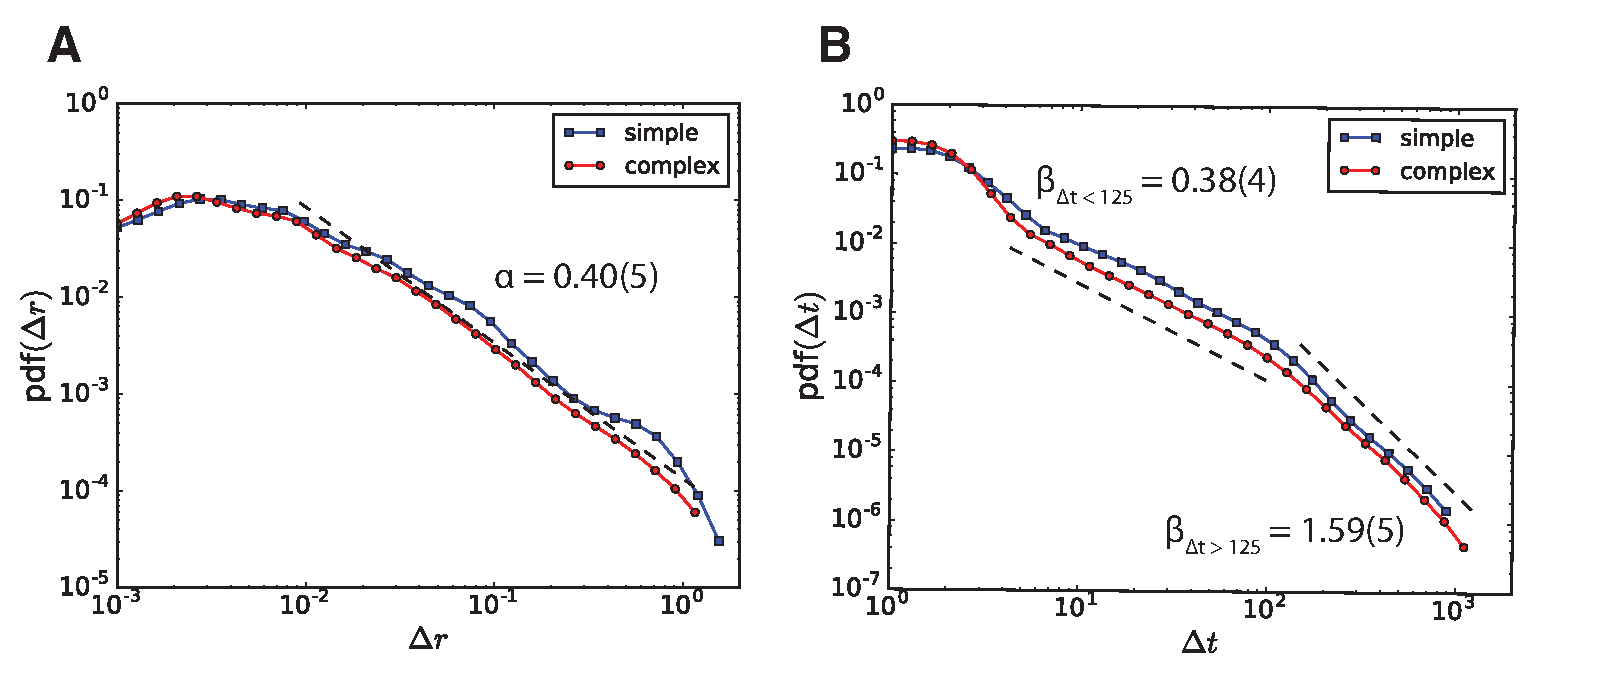
\includegraphics[width=17cm]{figures/CTRW.eps}
\caption{\footnotesize{{\bf A.} Probability density function of displacement $pdf(\Delta r) = \Delta r^{-\alpha -1}$ with $\alpha = 0.40(5)$ with a cut-off limited by the largest possible displacement, which is $\sqrt{k}$ with $k$ the number of joint probabilities to evaluate. {\bf B.}  Probability density function of waiting time $pdf(\Delta t) = \Delta t^{-\beta -1}$ with 2 regimes : $\beta_{\Delta t < 125} = 0.38(4)$ and $\beta_{\Delta t > 125} = 1.59(5)$. Distributions of $\Delta r$ and $\Delta t$ are equivalent for the simple and complex treatments.}}
\label{fig:CTRW}
\end{center}
\end{figure}

These results alone would suggest a super-diffusive search process, with mean square displacement (MSD) predicted to be,

\be
prediction_msd.
\ee

%$\sim t^{\mu}$ with  $\mu_{Levy} = 1$ \
%or super-diffusion $\mu_{CTRW} = \beta$ \cite{21,23}). Here, however, mean square displacement (MSD) decays as $\sim t^{\mu}$ with $\mu_{simple} =-0.23(2)$ and $\mu_{complex} =-\
%0.26(1)$ showing a much slower convergence than is generally expected.

However, the observed $MSD  =  XX$ rather exhibits a sub-diffusive process (see Figure \ref{}X for a comparison), hence suggesting a more subtle mental search, compared to a search process which would not optimize through the progressive integration of information \cite{} and use of memory \cite{}. We shall emphasize that the distribution of excursions is much more heavy-tailed than what has been computed as optimal search for foraging (i.e., $\alpha \approx 1$\cite{viswanathan_optimizing_1999,reynolds_displaced_2007,viswanathan_physics_2011}). \\

{\bf [A note on waiting times $\rightarrow$ maybe in discussion ?]} Note that waiting times  have been observed \cite{humphries_optimal_2014,song_modelling_2010}\\


{\bf [the subsection on performance could be here]}


We shall analyze the ``anomalous'' empirical mental search process and then proceed to explain how it deviates from the ``optimal search'' process (i.e., $\alpha = 1$). Deviations are characterized by (i) a much smaller power law exponent compared to other findings (ballistic process) and (ii) a much smaller (sublinear) MSD, which seems to contradict the ballistic process ($\alpha = 0.4 < 1$). 

Several mechanisms of cognition may explain such inconsistency.  Optimal foraging does not explicitly account for costs associated with continuous information intake, memory \cite{}, information processing \cite{}, and cognitive biases that may constrain the mental search process \cite{}. 


\subsection{Exploration beyond the currently known solution space vs. optimization using only current knowledge}

When participants start, they may have some preconceived notion of how variables might influence each other, yet they have no experience of the solution space (i.e., they know that they must find values between 0 and 1 for 8 (resp. 16) parameters for treatment 1 (resp. treatment 2) and that those parameters are constrained to add up to 1. Exploring beyond the already known solution space (i.e., convex hull) is critical, because without it, participants would just build one preconceived model and then stop.  Every other model that they consider, after having built the first model is by necessity beyond the cognitive frontier because at that point the cognitive frontier is a set containing only one member; the first model.  Later, as many models have already been explored, it is easier to stay within the cognitive frontier that is defined by the convex hull of all previous explorations and as time goes on it is cognitively increasingly more difficult to find novel regions that have not yet been explored.  

We are interested in proposed models, which go beyond the solution space known at iteration $i$. If twice $\langle D_{jsd,i} \rangle$, the average distance of solution $j$ compared to all previous solutions $i < j$, is larger than $ max(D_{jsd})$ the maximum distance between 2 solutions in $iterations = \{1,...,i\}$, then the new proposed model {\it {\bf incorporates causal hypotheses and conditional independence assumptions, which are not entailed by previously explored models}} and contributes to the enlargement of the currently explored joint-hypotheses space. To measure how much a proposed model is explorative, versus exploitative of causal and conditional independence structures, we define the ratio:

\begin{equation}
EE_{j} = \frac{2 \langle D_{jsd,j} \rangle}{max(D_{jsd,1,...,j})}.
\end{equation}

For $EE < 1$, the individual is choosing an exploitative solution, that lies within the boundaries of the convex hull of already explored solutions. For $EE \approx 1$, the proposed solution is on -- or close to -- the boundaries, and for $EE > 1$, the proposed solution is outside the convex hull, and therefore explorative. The larger $EE$, the more explorative the proposed solution. For both 3-node and 4-node BN treatments,  the number of explorative moves is over all people much larger than exploitative ones :  $5416$ vs. $1873$ (resp. $6260$ vs. $4689$). It is of course critical to know how exploration and exploitation vary over time. It is optimal, in fact necessary to explore a lot in the beginning, when not much is known about the space or its payoffs, but it is diminishingly fruitful to explore towards the end of the game, for three reasons: 1) because towards the end it is harder to find truly new solutions as one's creativity is more taxed to find further unexplored patterns, 2) because it may seem less likely that the novel solutions--once they are found--will be improvements and 3) because even if improvements are as likely as losses, it is harder to make up for losses towards the end and thus risk is affected. The structure here is as in a work-retirement game wherein it makes sense to speculate and take large risks earlier in one's career when the benefits can have immense impacts on one's whole life span and it makes sense to be conservative later in one's career, where losses can not be easily made up for and most of the opportunities appear to have already been considered, whether this is truly the case or not.    
%{\bf yes! I very much agree and one could in fact work out some equilibrium or optimal exploration as a function of time and cognitive costs as well as expected benefit from exploration (itself perhaps subject of experiential learning and a model of its own) ...I'm not saying that we should, but we may mention it as a possibility of something that an economist, or a theorist of incentivized optimal learning might be interested in doing. }

An exact equilibrium path of allocation between exploitation and exploration could be worked out, that logically should start with maximum and speedy exploration of the space--exactly as speedily as hypotheses can be tested with new observations and not speedier.  This speedy exploration should be the policy in the beginning, when the mental state is complete ignorance.  The game should end in coming as close as possible to understanding the process, such that any risk of further exploration is no longer worth the expected life-time benefits and exploration should completely stop. This is the time when optimization should be completely exploitative fine-tuning.    
 



\begin{figure}[h!]
\begin{center}
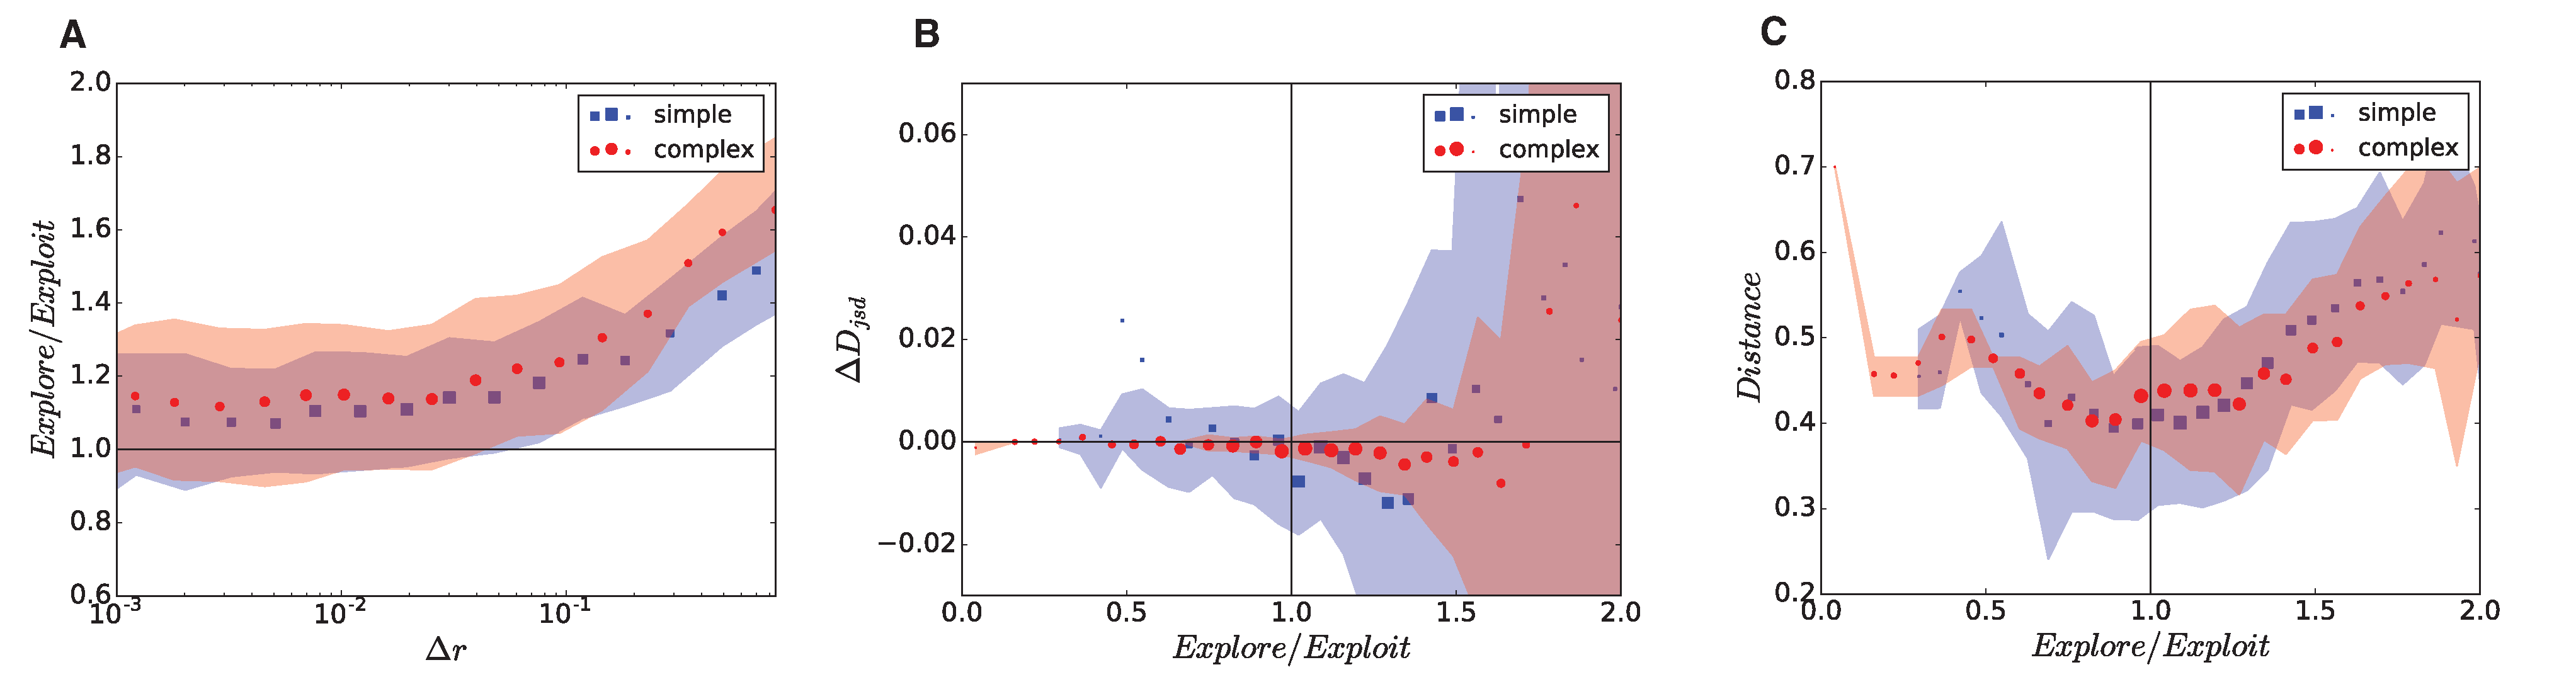
\includegraphics[width=18cm]{figures/EE.eps}
\caption{{\bf A.} Explore / Exploit ($EE$ )as a function of displacement $\Delta r$. {\bf B.} $\Delta D_{jsd}$ as a function Explore / Exploit: Improvement seems better for $EE \approx 1.4$. {\bf C.} $D_{jsd}$ as a function of $EE$: As distance gets smaller, a balance around $EE = 1$ seems to be reached.}
\label{fig:pdf_return}
\end{center}
\end{figure}

\subsection{Return to previously visited sites}
We also find that individuals tend to repeatedly return to previously visited solutions. The probability distribution is found to follow a power law with exponent $\gamma \approx 1.5$  (see Figure \ref{fig:memory}B)

\subsection{Recency of memory}
Memory plays a central role in recombining multiple previously explored models into new ones. We find strong influence of a focal model on subsequent models. On average over all participants in each treatment, influence $I$ decays as $I \sim t^{-\chi}$ with $\chi = 0.48(2)$ ($p < 0.01$ and $R > 0.32$)  (Figure \ref{fig:2}B). Because the time decay exhibits a power law with exponent $\chi < 1$, on average, models proposed in the past never vanish from memory, and may be reused or inspire future models. If we assume that the rate of proposed models remains roughly constant  over time for some participant, as time passes it gets statistically harder to come up with novel solutions ``because mental constructions are imprinted by past experience'' and the cognitively low hanging fruits as well as all of their combinations are used up, leaving less and less intuitive solutions in the unexplored space of models. Often--as in the Monty Hall example--the true processes of stochastic influence and their observational consequences are highly counter-intuitive.  


\begin{figure}[h!]
\begin{center}
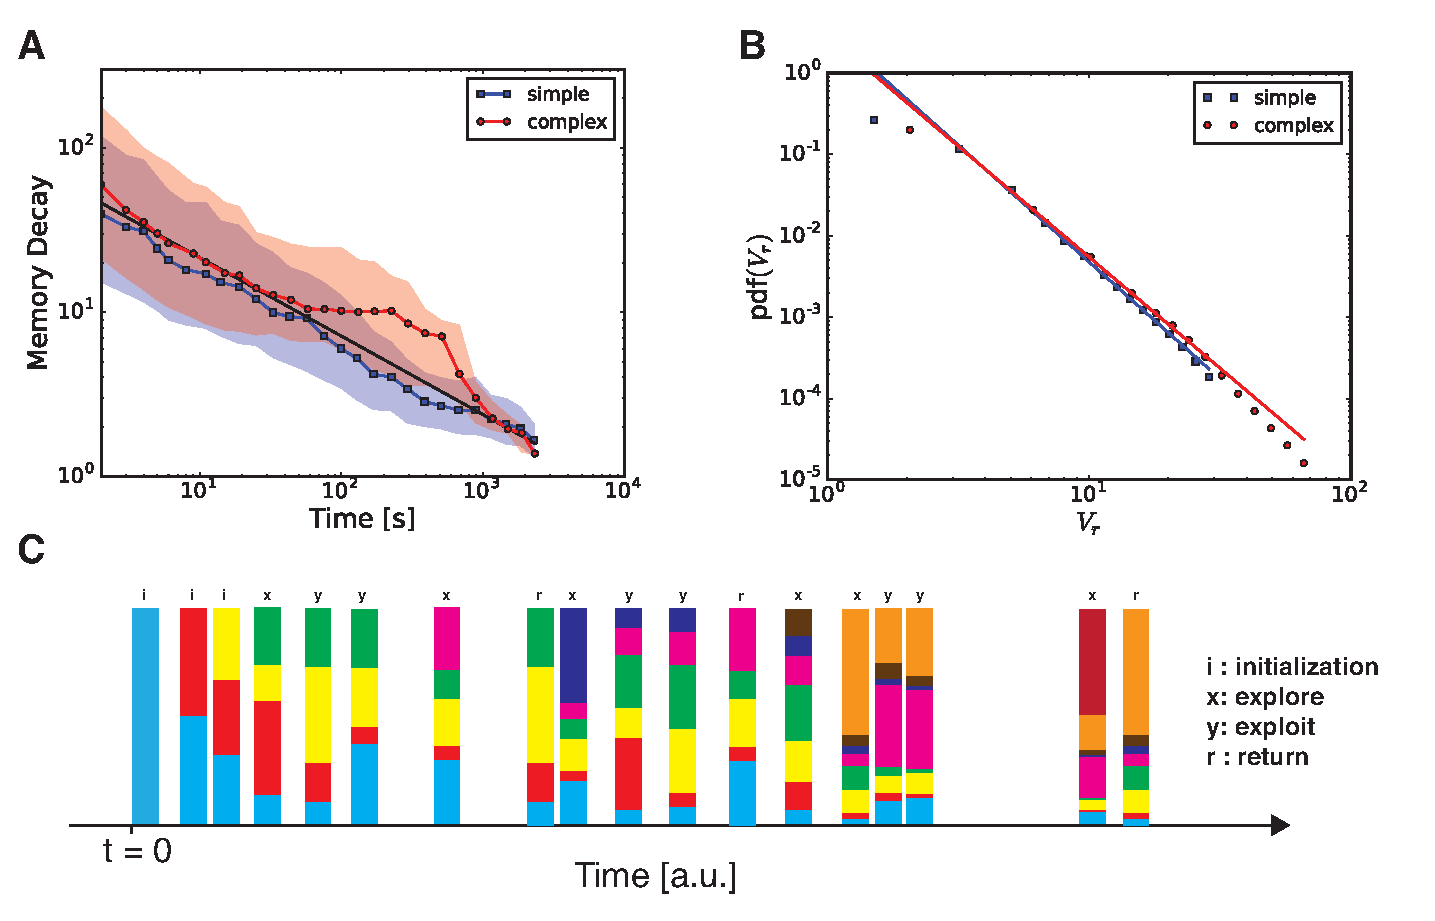
\includegraphics[width=15cm]{figures/memory.eps}
\caption{{\bf A.} Influence of a model proposed at time $t$ in subsequent models. The influence is computed as 1/distance between the focal model and subsequent models. On average over all participants in each treatment, influence $I$ decays as $I \sim t^{-\chi}$ with $\chi = 0.48(2)$ ($p < 0.01$ and $R > 0.32$). This result shows that memory is important, with implications for the convergence. {\bf B.} Return to previously visited sites : $\mathrm{pdf}(V_r) \sim {V_r}^{- \gamma -1}$, with $\gamma_{simple} = 1.6(1)$ and $\gamma_{complex} = 1.5(1)$ $\rightarrow$ tendency to return to previously visited sites : This goes against the imperative to visit new sites (maximize $S_T$) in order to reduce $D_{min}$ (c.f. Figures \ref{fig:Dmin_vs_St}B and \ref{fig:Dmin_vs_St}C). Moreover, given the large number of sites [$10^{8}$ (resp. $10^{16}$) in the simple (resp. complex) case], it is remarkable that participants tend to return to exactly the same (tiny) spots. This suggests some stickiness of memory. {\bf C.}  Schematic representation of remix dynamics. The color bars show the proportion (i.e., $1/d$) of previously proposed solutions in solution proposed at time $t$. New colors are introduced 	tosignal exploration. From time to time, individuals return to previously visited solutions (signaled by $r$).}
\label{fig:memory}
\end{center}
\end{figure}


\clearpage


%\begin{figure}[h!]
%\begin{center}
%%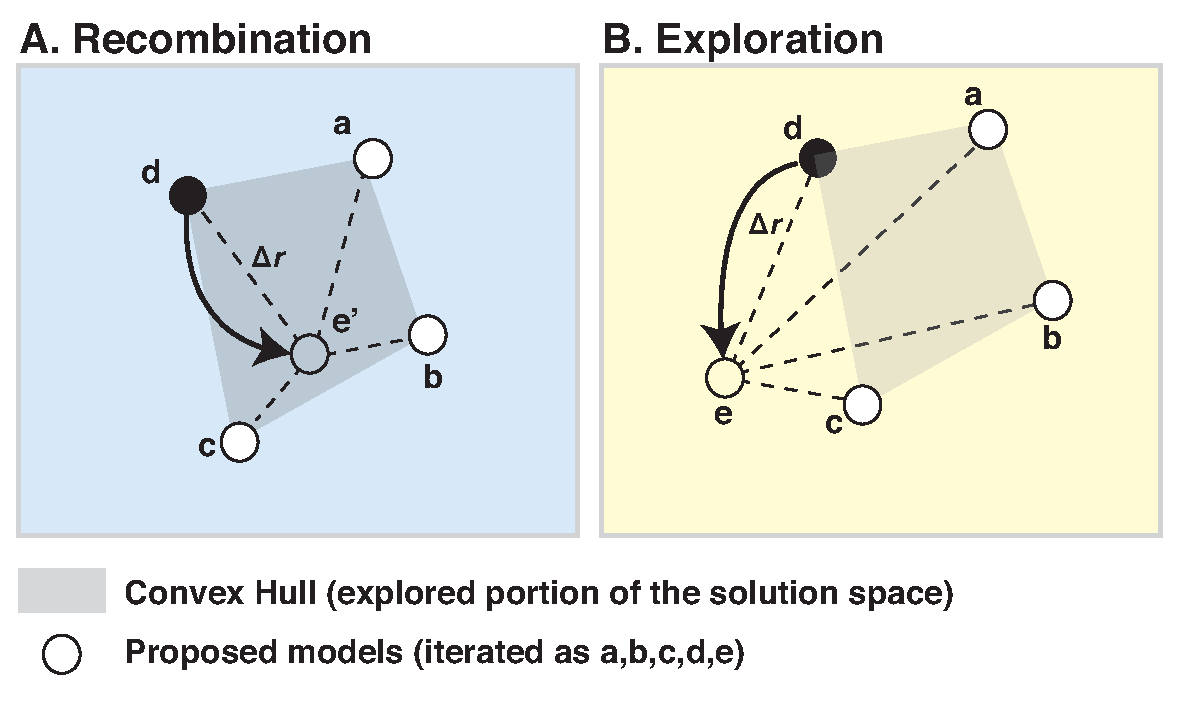
\includegraphics[width=12cm]{figures/figure2.eps}
%\caption{\footnotesize{move patterns}}
%\label{fig:move_patterns}
%\end{center}
%\end{figure}



%{\bf A.} Average Jensen-Shannon Distance $\langle D \rangle$ decays as a function of time as $\sim t^{\nu}$ with $ \nu \approx -0.15(1)$ indicating a very slow convergence to the true model {\bf [indicate $t_0$s and what their values may mean]}. 

%\begin{figure}[h!]
%\begin{center}
%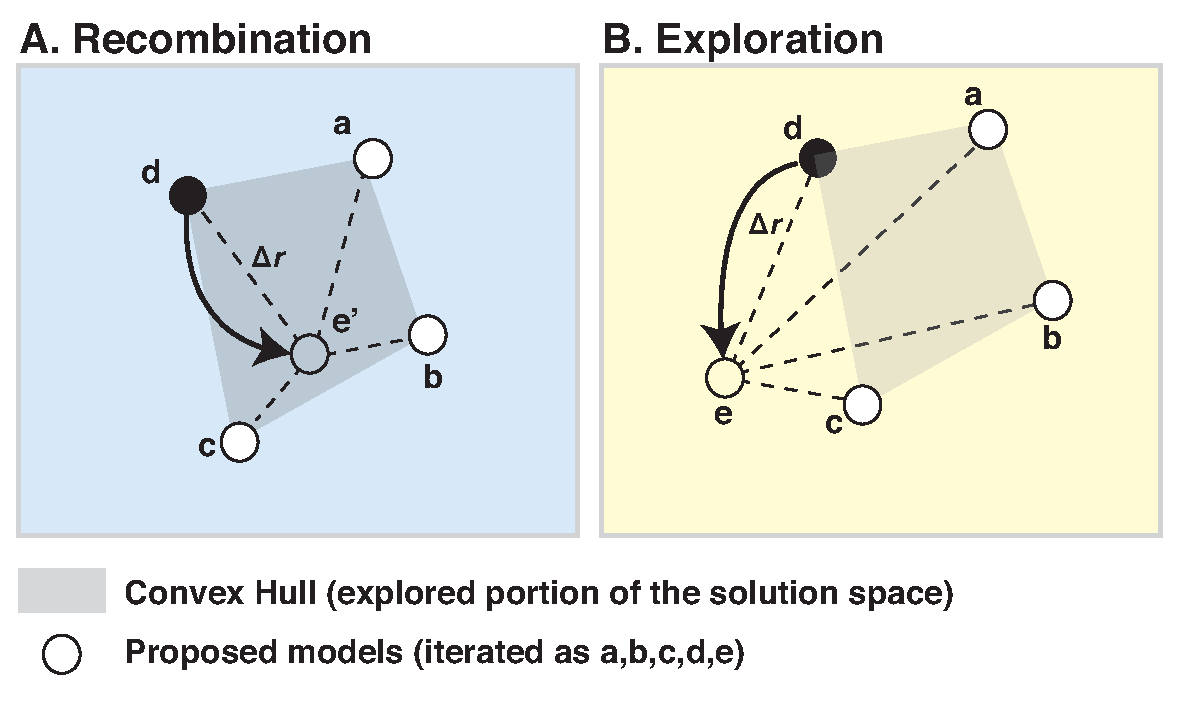
\includegraphics[width=12cm]{figures/figure2.eps}
%\caption{\footnotesize{Simplified diagram of exploration and recombination on a plane: {\bf A. Recombination:} iteration {\bf e'} does not incorporate new information. It is a convex combination of all previous proposed solutions (i.e., $\{a,b,c,d\}$).  {\bf B. Exploration:} the average distance between iteration {\bf e} and all previous iterations is larger than half of the maximum distance between any previous proposed solutions. Exploration is not memoryless: {\bf e} is closer to {\bf c} and {\bf d} than {\bf a} and {\bf b}. }}
%\label{fig:2}
%\end{center}
%\end{figure}


%\subsection{Memory, Return to previously visited sites \& Recombination}


%\begin{figure}[h!]
%\begin{center}
%%\includegraphics[width=16cm]{figures/Figure1.eps}
%\caption{\footnotesize{{\bf A.} return to previously visited sites : $\mathrm{pdf}(V_r) \sim {V_r}^{- \gamma -1}$, with $\gamma_{simple} = 1.6(1)$ and $\gamma_{complex} = 1.5(1)$ $\rightarrow$ tendency to return to previously visited sites : This goes against the imperative to visit new sites (maximize $S_T$) in order to reduce $D_{min}$ (c.f. Figures \ref{fig:Dmin_vs_St}B and \ref{fig:Dmin_vs_St}C). Moreover, given the size of the parameter space [the simplex of dimension $10^{8}$ (resp. $10^{16}$) in the simple (resp. complex) case], it is remarkable that participants tend to return to exactly the same infinitesimal spots in this space. This suggest memory dependent stickiness. {\bf B.} Influence of a model proposed at some time, $t$ in subsequent models at some $t +s$, with $s \geq 1$. The influence is computed as 1/distance between the focal model and subsequent models. On average over all participants in each treatment, influence $I$ decays as $I \sim t^{-\chi}$ with $\chi = 0.48(2)$ ($p < 0.01$ and $R > 0.32$). This result shows that the importance of a memory decays slowly, with implications for the convergence of beliefs to the processes that are the content of those beliefs.}}
%\label{fig:3}
%\end{center}
%\end{figure}

\begin{figure}[h!]
\begin{center}
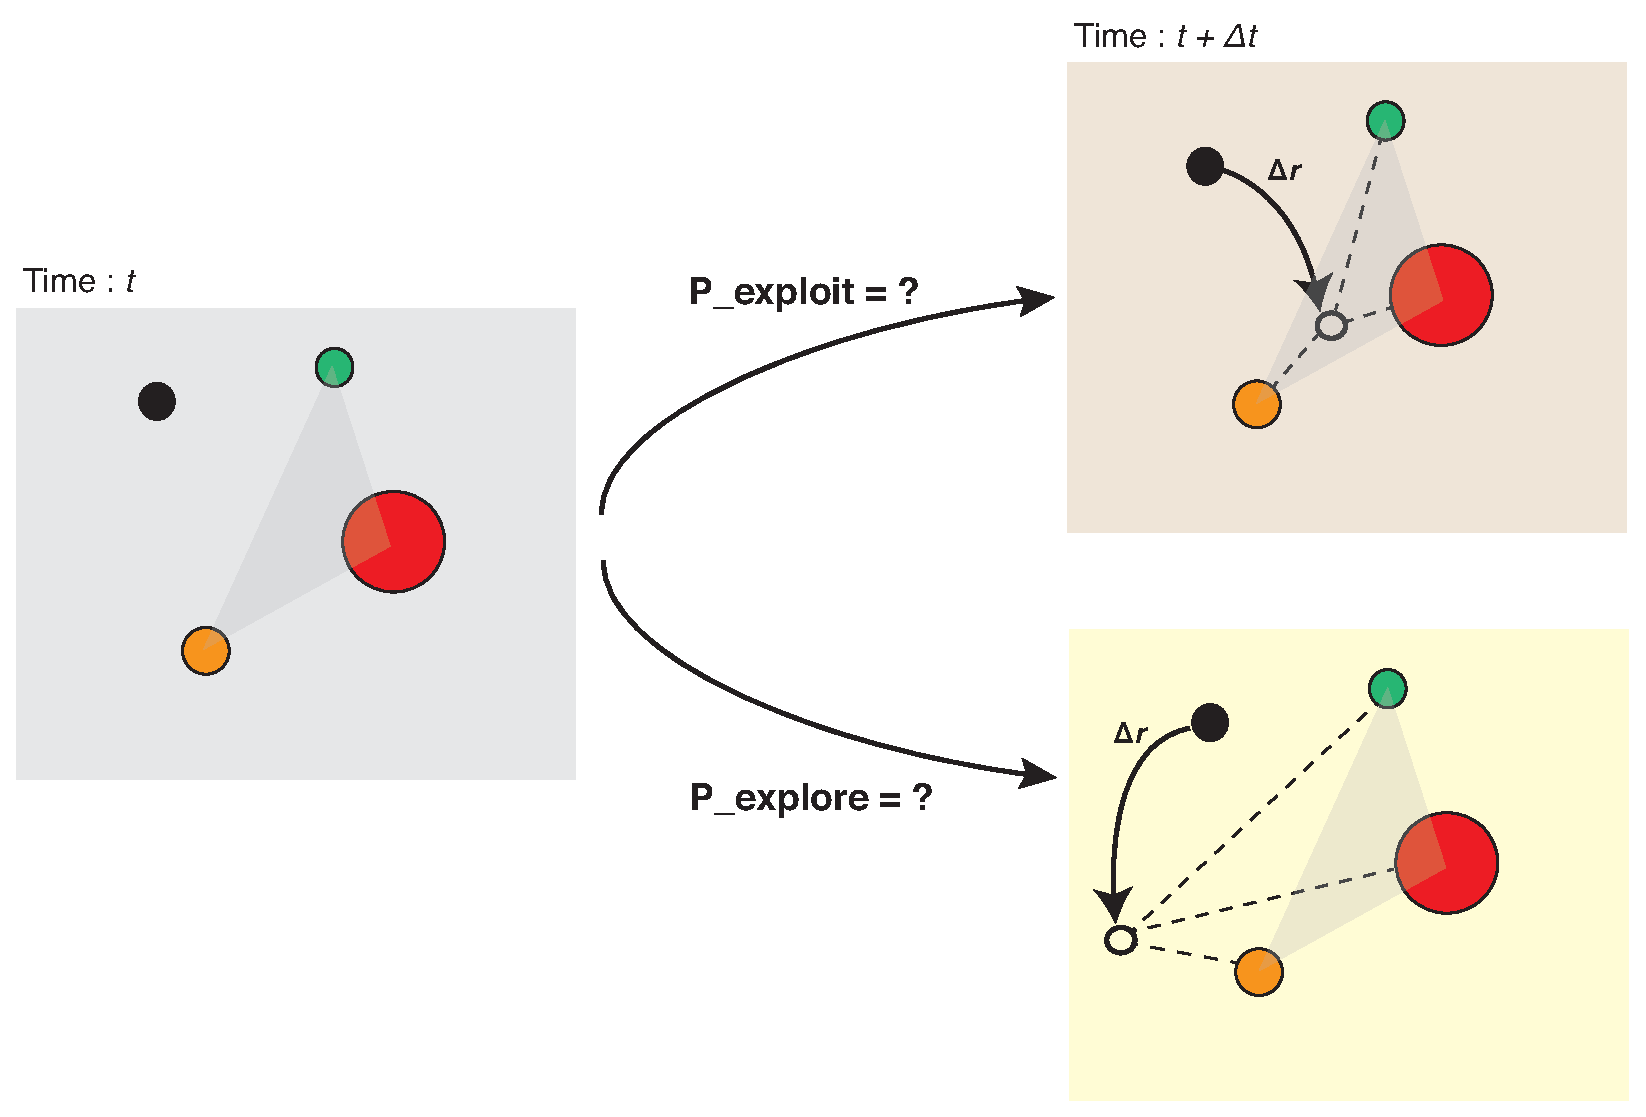
\includegraphics[width=10cm]{figures/schematic_displacement.eps}
\caption{2-dimensional schematic description of the {\it L\'evy flying mind} model ({\bf ``Proportional Attraction"}): At each time step, the individual must choose between remaining in the solution envelope that has already been explored and exploring outside the currently known solution envelope.  We assign some probability $p$ (a number between 0 and 1) to the participant's decision of staying in the explored envelop and probability $1-p$ to the decision to explore outside that envelop.  If it is harder to find solutions that offer a balanced re-combination of previous solutions than to think out-of-the-box and propose solutions outside of the current solution envelope, then $p < \frac{1}{2}$ else $p \geq \frac{1}{2}$.}
\label{fig:schematic}
\end{center}
\end{figure}










\subsection{Implications of Memory and Exploration on Performance}
Individuals deploy {\it exploration}, {\it exploitation}, and {\it return} strategies in order to get closer to the best solutions (i.e., factorizations of the joint distribution that are indistinguishable from the true model). Each move may lead to improvement (i.e., reduction of cognitive distance to the true model) or, on the contrary, to dis-improvement. 

We find that displacement has an influence on improvement. As one could surmise, small displacements can only bring marginal improvement, while larger displacements bring more opportunities for improvement, yet at the cost of potential short-term losses that may be quite large. Large displacements ($\Delta r > 0.2$) can destroy performance, but also have the potential to improve understanding for all future periods. Figure \ref{fig:vs_dr} shows the evolution of the distance to the true model $D$ as a function of displacement $\Delta r$. The distance scales as $D \sim {\Delta r}^{\mu}$ with $\mu_{simple} = 0.88(1)$ [resp. $\mu_{complex} = 082(2)$]. For $\Delta r > 0.2$, $D$ uncertainty quickly balloons, but rather positive, reflecting the {\it cost} of making ``wild'' innovations. 

There is no clear relation between time spent on taking the decision to move and performance {\bf [show $\Delta D_{jsd}$ versus $\Delta t$] if relevant: question here is the functional form of how time spent on cognitive processing leads to better or worse results.}.

While there is no clear relation between time spent between moves and performance {\bf [$\Delta D_{jsd}$ versus $\Delta t$]}, the decision to make a larger displacement takes more time. For $\Delta r < 0.2$, the processing time before a displacement decision is made scales as $\Delta t \sim \Delta r^{\gamma}$ with $\gamma_{simple} = 0.11(1)$ [resp. $\gamma_{complex} = 0.13(1)$]. For $\Delta r > 0.2$, the processing times before a displacement decision is taken get disproportionally long (up to tens of seconds on average for a displacement of 0.7 (i.e., $\approx 25\%$ of the maximum displacement distance). On both panels, blue and red areas show the $25^{th}$ percentile confidence intervals.

The minimum distance $D_{min}$ (between the best model and the true model) exhibits scaling as a function of the number of distinct sites visited $S_{T}$. $D_{min} \sim S_{T}^{\gamma}$ with resp. $\gamma_{simple} = -0.20(4)$ and $\gamma_{complex} = - 0.13(3)$. {\bf C.} The logarithm of number of visited sites is a linear function of the logarithm of time $t$. Hence, the number of distinct visited sites is a predictor of the minimum distance $D_{min}$ achieved at time $t$. The result also holds for groupings with averaged cognitive distances.


\begin{figure}[h!]
\begin{center}
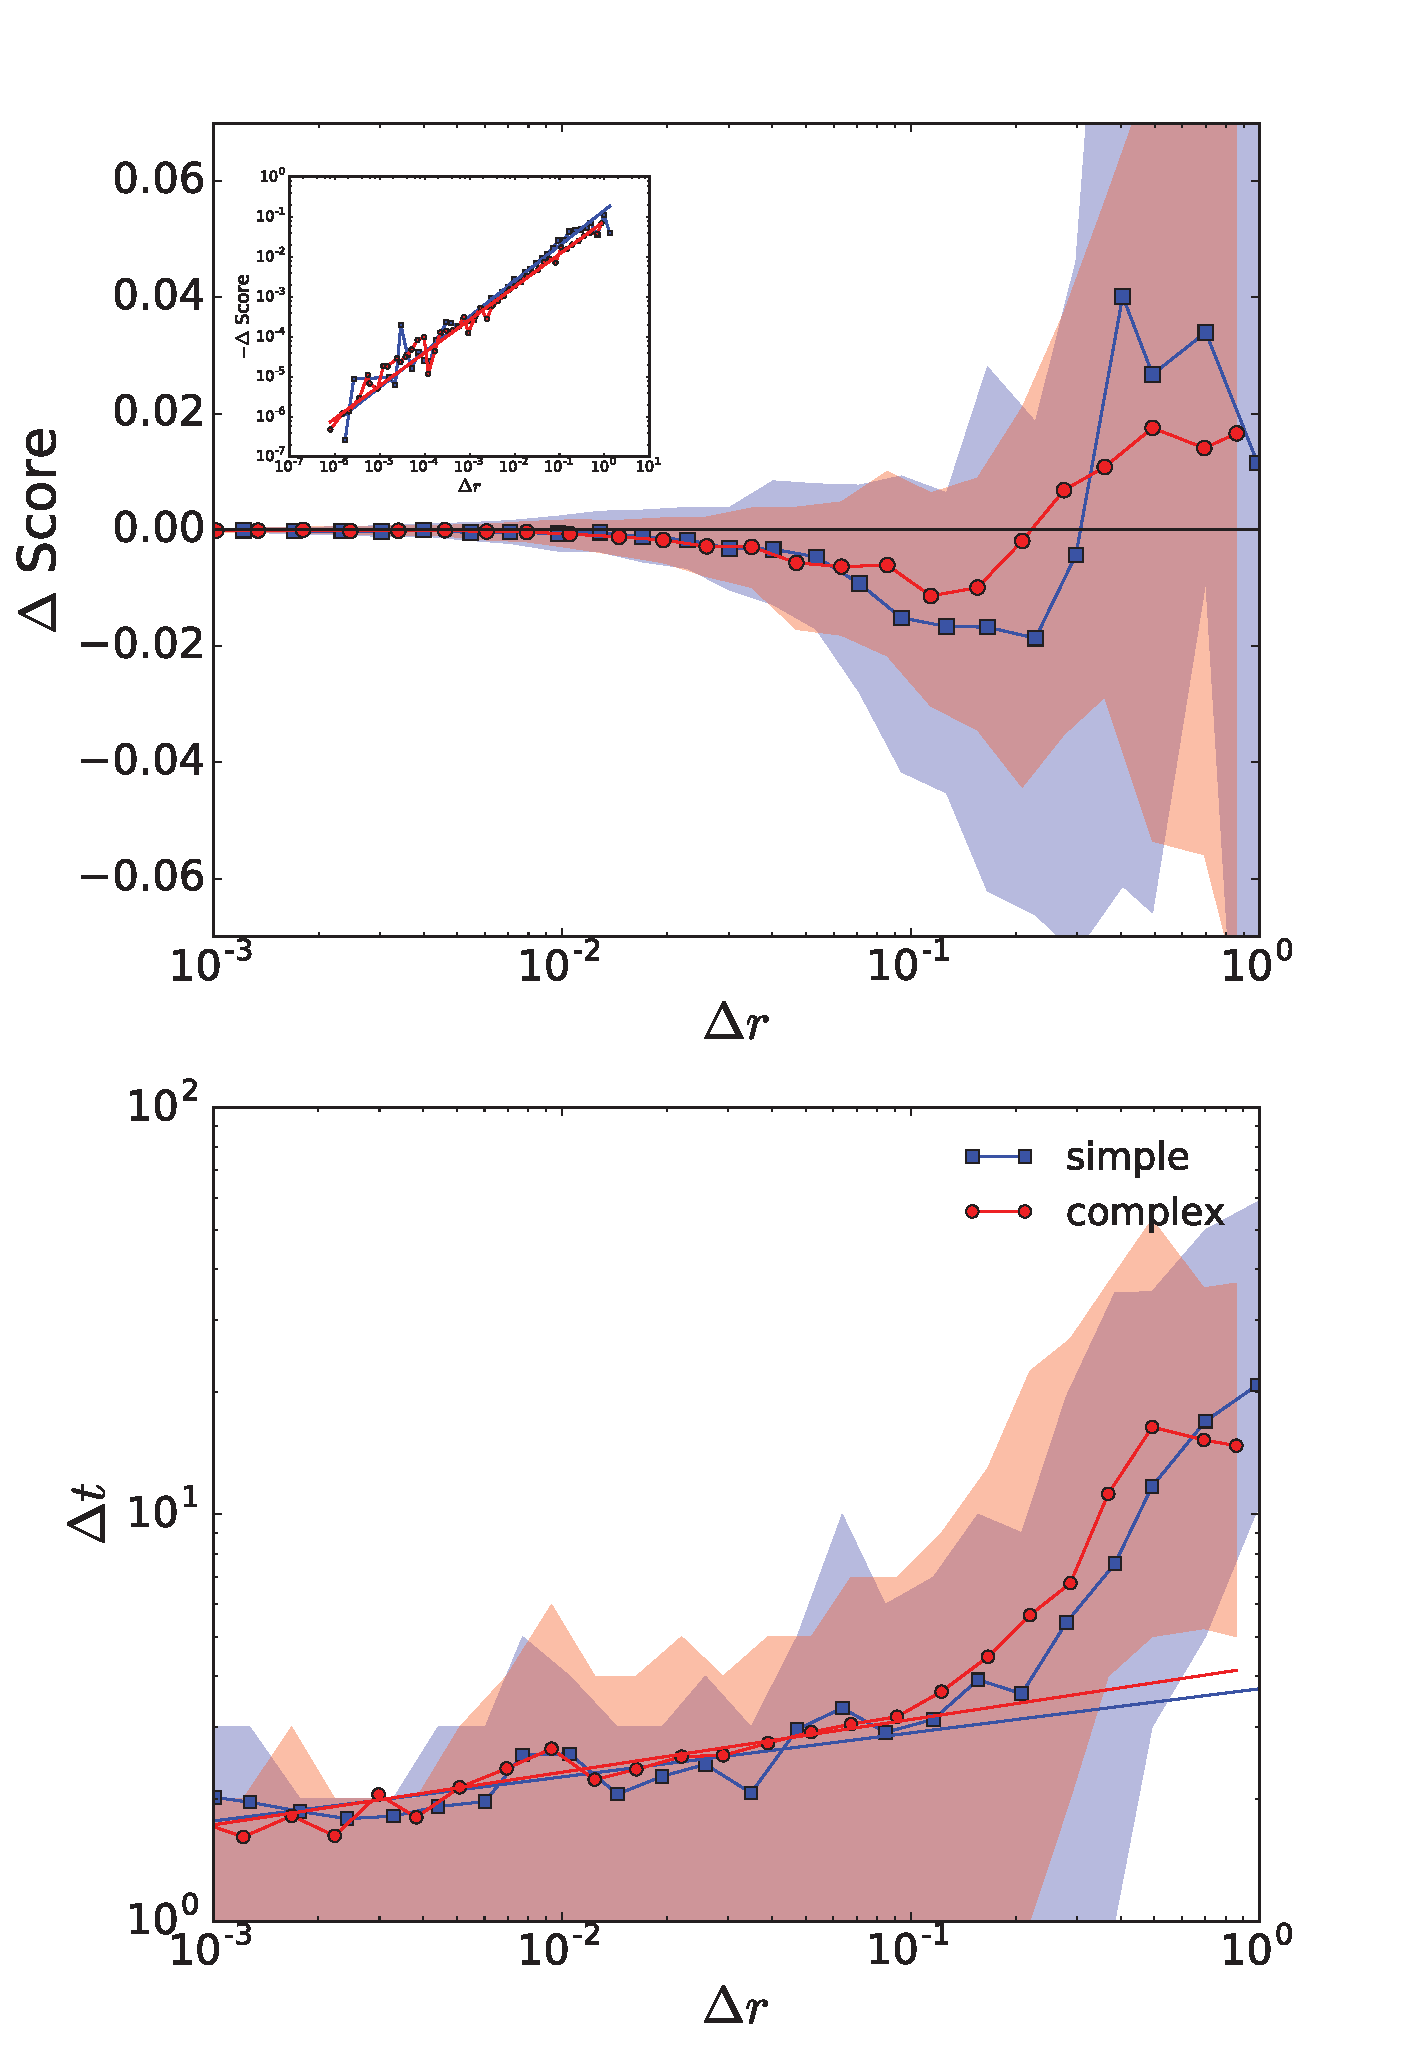
\includegraphics[width=11cm]{figures/vs_dr.eps}
\caption{{\bf A.} Evolution of the distance to the true model $D$ as a function of displacement $\Delta r$. The distance scales as $D \sim {\Delta r}^{\mu}$ with $\mu_{simple} = 0.88(1)$ [resp. $\mu_{complex} = 082(2)$]. For $\Delta r > 0.2$, $D$ becomes quickly highly uncertain, but rather positive, reflecting the {\it cost} of the making ``wild"displacements. {\bf B} For $\Delta r < 0.2$, the waiting time before a displacement decision is made scales as $\Delta t \sim \Delta r^{\gamma}$ with $\gamma_{simple} = 0.11(1)$ [resp. $\gamma_{complex} = 0.13(1)$]. For $\Delta r > 0.2$, the waiting time before a displacement decision is taken get disproportionally long (up to tens of seconds on average for displacement of 0.7 (i.e., $\approx 25\%$ of the maximum displacement distance). On both panels, blue and red areas show the 25th percentile confidence intervals.}.
%\caption{Scaling relation between $\Delta t$ and $\Delta r$ for the simple (A) and complex (B) treatments. The functions are similar for both treatments [resp. $\sim 0.44(2)$ ($p < 0.01$ , $r = 0.39$) and $\sim 0.47(2)$ ($p < 0.01$ , $r = 0.36$)]. {\bf Actually, one may see this figure differently : scaling $\Delta t \sim {\Delta r}^{0.2}$ for $\Delta r < 0.2$ and another (unknown) regime for $\Delta r > 0.2$ with waiting time getting disproportionately long $\rightarrow$ This may highlight the processing costs associated with a big jump.}}
\label{fig:vs_dr}
\end{center}
\end{figure}


\subsection{Computer vs. Optimal Foraging vs. Human Performance}

\begin{figure}[h!]
\begin{center}
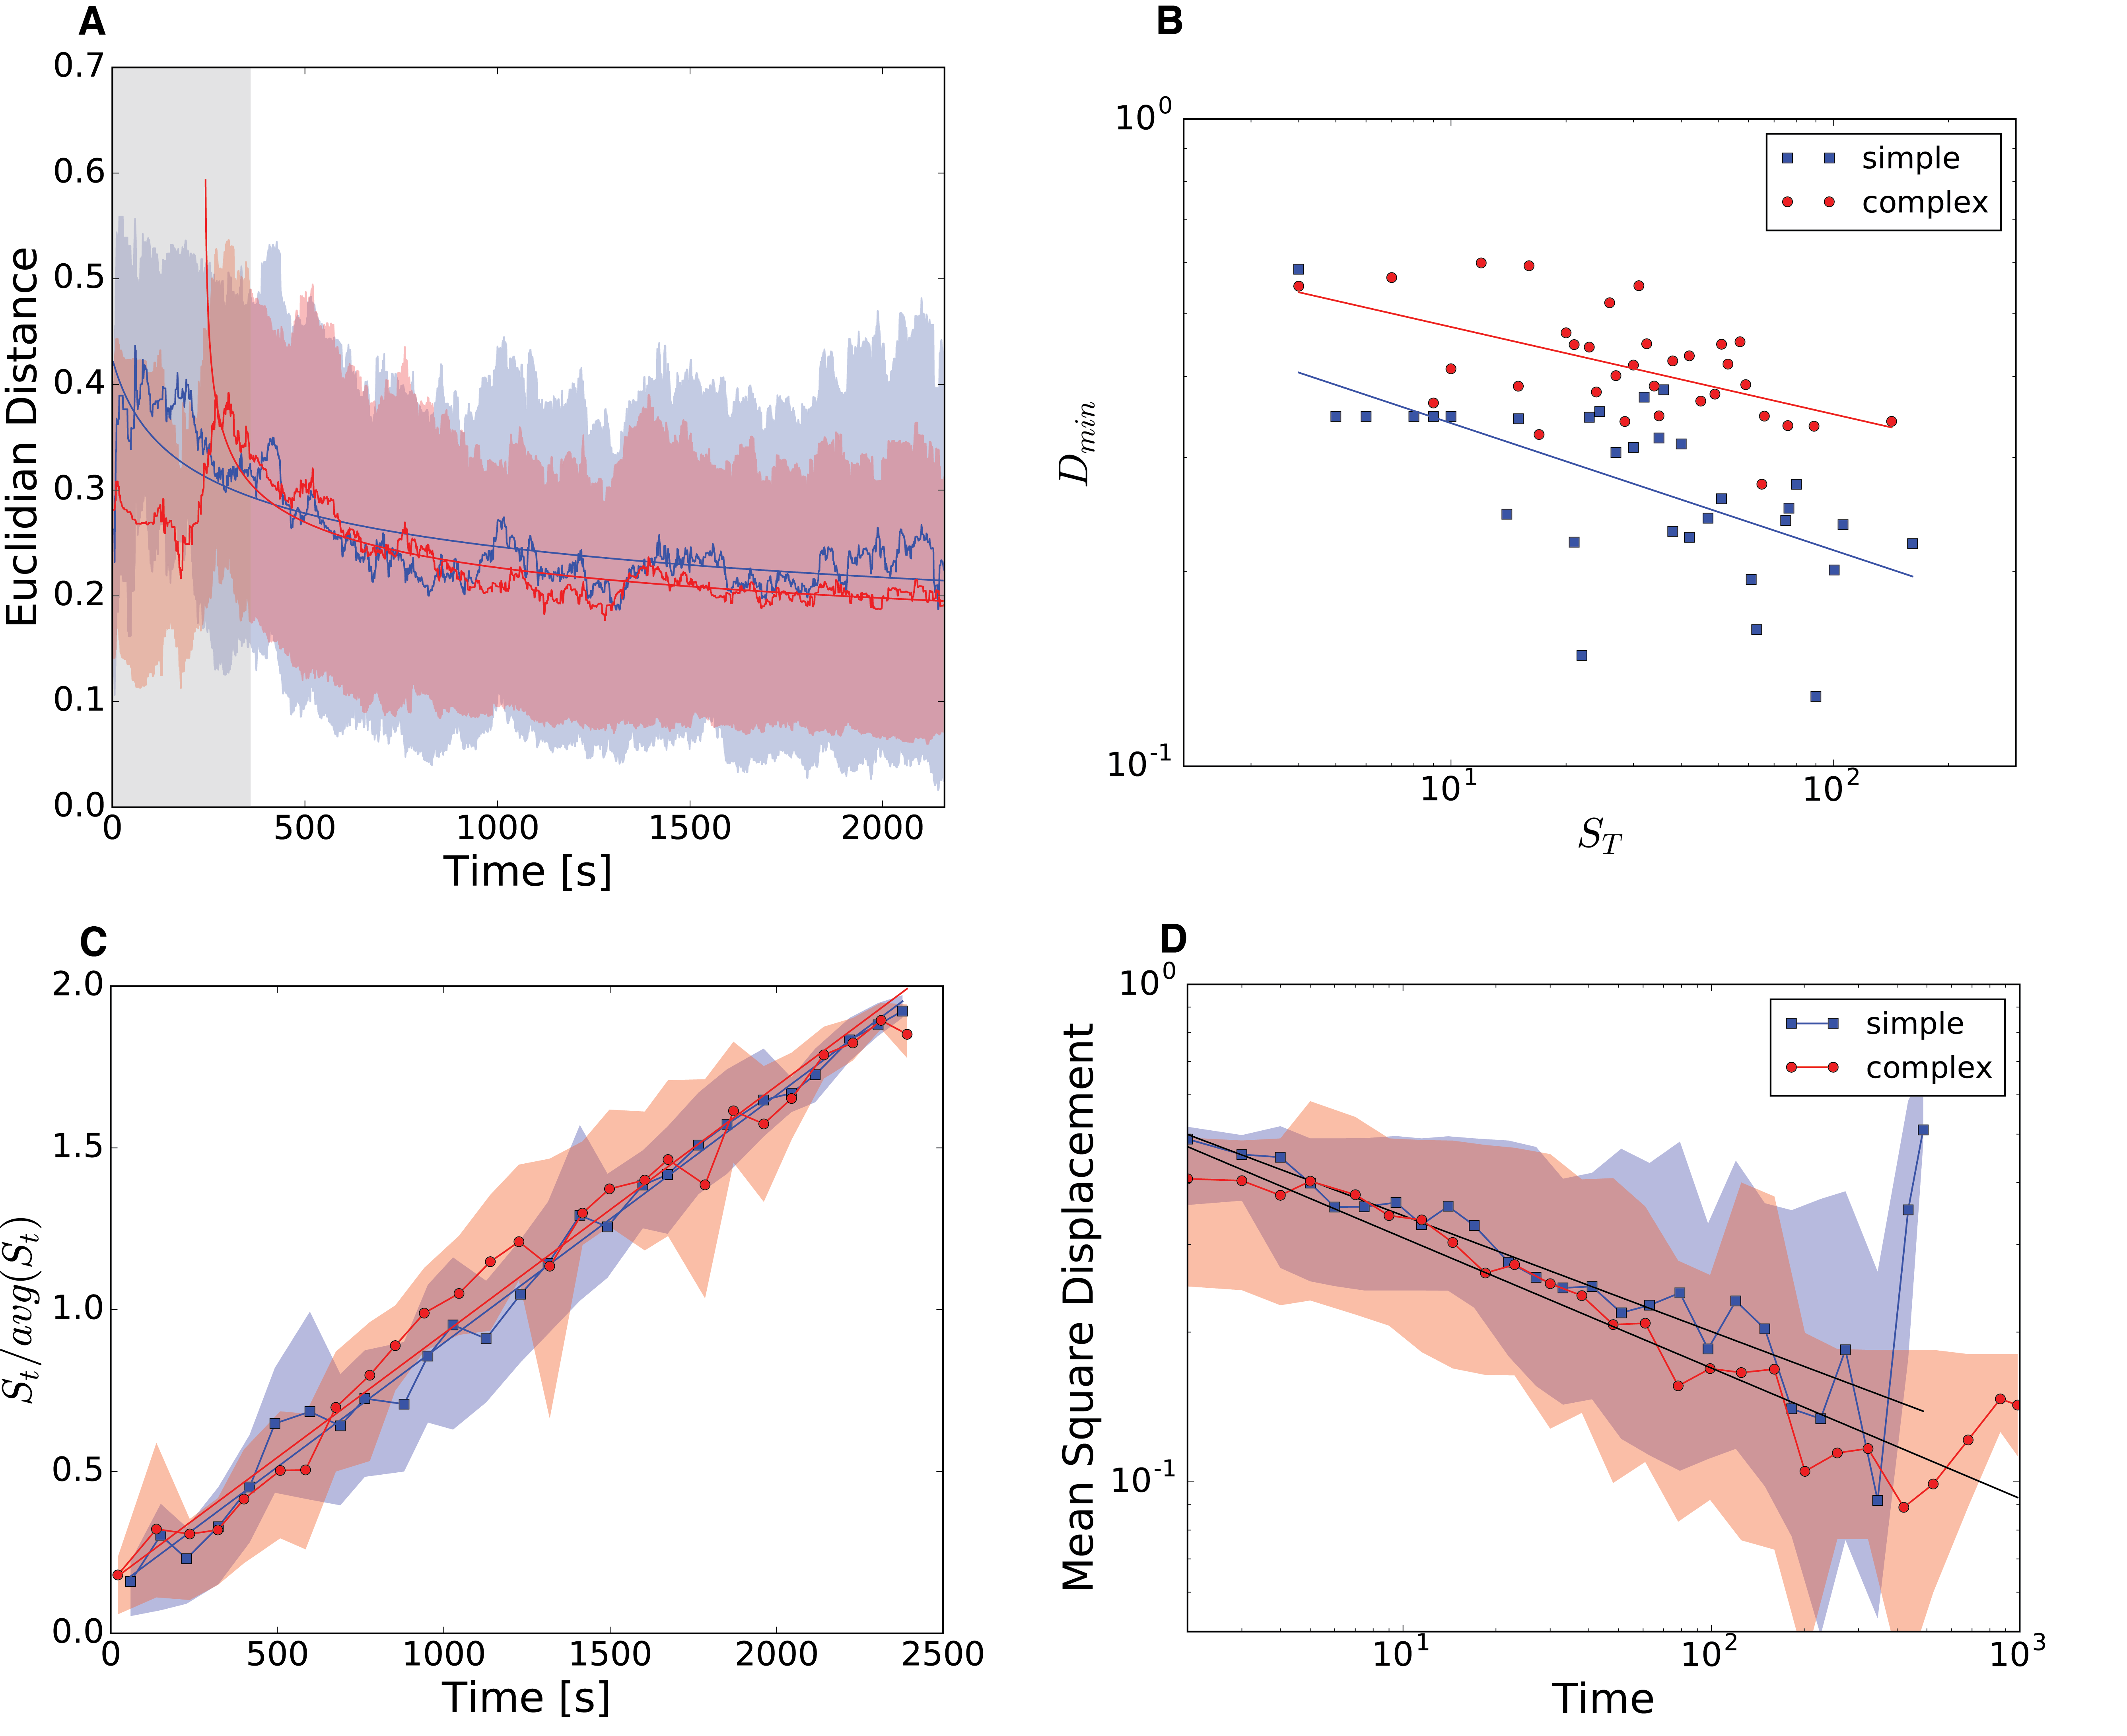
\includegraphics[width=16cm]{figures/Dmin_vs_St.eps}
\caption{{\bf A.} Minimum Jensen-Shannon distance $D_{min}$ (between the best model and the true model) exhibits a scaling as a function of the number of distinct sites visited $S_{T}$. $D_{min} \sim S_{T}^{\gamma}$ with resp. $\gamma_{simple} = -0.20(4)$ and $\gamma_{complex} = - 0.13(3)$. {\bf B.}  The number of visited sites over time $S_t$ is a linear function of time $t$. Hence, the number of distinct visited sites is a predictor of the minimum distance $D_{min}$ achieved. The result also holds for average distance. {\bf C.}  Mean square displacement (MSD) decays as $\sim t^{\mu}$ with $\mu_{simple} =-0.23(2)$ and $\mu_{complex} =- 0.26(1)$ showing a slow convergence (on the contrary of a normal L\'evy flight / CTRW, which is characterized by respectively diffusion $\mu_{Levy} = 1$ or super-diffusion $\mu_{CTRW} = \beta$ \cite{21,23}). All colored areas show the 25th percentile confidence intervals.}
\label{fig:Dmin_vs_St}
\end{center}
\end{figure}


{\bf [here, we should have a simulation of computer resolution process by a computer (Johannes you did this already), as well as a simulation of optimal foraging (displacement following a power law distribution with exponent 1)]}


\subsection{Waiting Times}

economic aspects (i.e., time is the scarce ressource)

\subsection{The Role of Incentives in Experimental Economics}

Experimental Economists have long differenciated themselves from experimenters in psychology and cognitive science, by rewarding their experimental participants directly for their efforts, such that better performance leads to higher expected payoffs from the laboratory experiment. The theories that are tested often mirror the conditions of a simplified but at least in one aspect realistic market environment and incentives are a natural and important part of such environments. It should be noted that outside of the laboratory, most cognitively demanding tasks have the characteristic that the quality of one's understanding is directly related to one's payoffs. This is true in the case of food search and it is true in the case of investment in a set of causally related securities, which the experiment from which we have our data seeks to mimic. Even in computational, agent based models, an agent must have some fitness or utility function that it has the intention to maximize \cite{dennett1989intentional} and in real human lives, money is theoretized to fulfill this fucntion well and this assumption has been tested in many other experiments and the evidence is largely consistent with this hypothesis.  The evidence has been summarized in a classic article \cite{smith1993} and the issue has been largely put to rest after that.    \cite{loewenstein99} gives a detailed critique on the external validity of experimental economics, where he acknowledges that some special institutions such as stock markets may be accurately represented through carefully structured experimental incentives. At the same time, the paper warns, some societal phenomena may not be well approximated enough through experimental economic methodology to have much external validity.   


\subsection{The Role of Incentives in our specific experiment}

The Becker-Degroot Marshak Method, in particular, is a workhorse in experimental economics, as a true valuation revealing incentive scheme for random goods \cite{ortega2018mitigating, tymula2016flexible, diro2016effect}. 
They way that this works is that a lottery is defined; in our case the lottery is that if some variable will take on the value H then playing the lottery will have a payoff of \$ 1 and if the variable takes on the value L, playing the lottery will payoff \$ 0.  In our case, whatever value the variable takes on is probabilistically determined by whatever values two or three covariates have already taken on and those values, but not their probabilistic influences, are known.  So, conditional on some other variables' known values, the lotery is regarding the hidden value of some variable.  Now, given our lotery, the Becker-Degroot Marshak Method is as follows.  Participants are stating in essence what they believe this lottery is worth.  By stating, for example, through their setting of parameters, that the probability of the variable taking on H is 0.5, then this is the same as stating that the lottery is worth \$ 0.5.  Then the computer decides an offer price and if this price is \$ 0.6, the participant is immediately rewarded 60 cents, however if this random offer price is 40 cents, then the participant ends up playing the lottery and is awarded \$ 1 if the variable takes on the value H and otherwise \$ 0.  This incentive scheme has been shown to be truth revealing of peoples beliefs regarding the value of some good (any good) and in particular the believed value (in this case just the probability expressed in cents) of some lottery.  Since this is repeated 30 times, at maximum stake are 30 dollars and everage payoffs were around \$14.  A \$ 5 dollar showup fee was also paid, so average total take-home pay for the participants was \$ 19.    

\cite{irwing98} empirically shows that steep incentive differences for better results might be necessary for cases in which individuals must seek out the solution to a problem and in which it isn't easy to deduce.  How steep are the differences in incentives in our experiment, are they steep enough, given the complexity of the problem at hand?  We can not definitively answer that question and through cognitive cost explanations the slow learning might be partially or in total a result of not sufficiently steep incentive differences. More work would be needed to know if it is the insufficiently steep incentives or the sufficiently steep cognitive costs that determine the characteristics of the learning curve in our experiment.     

%\section{Model of L\'evy Walks/Flights in cognition incorporating memory}


\begin{figure}[h!]
\begin{center}
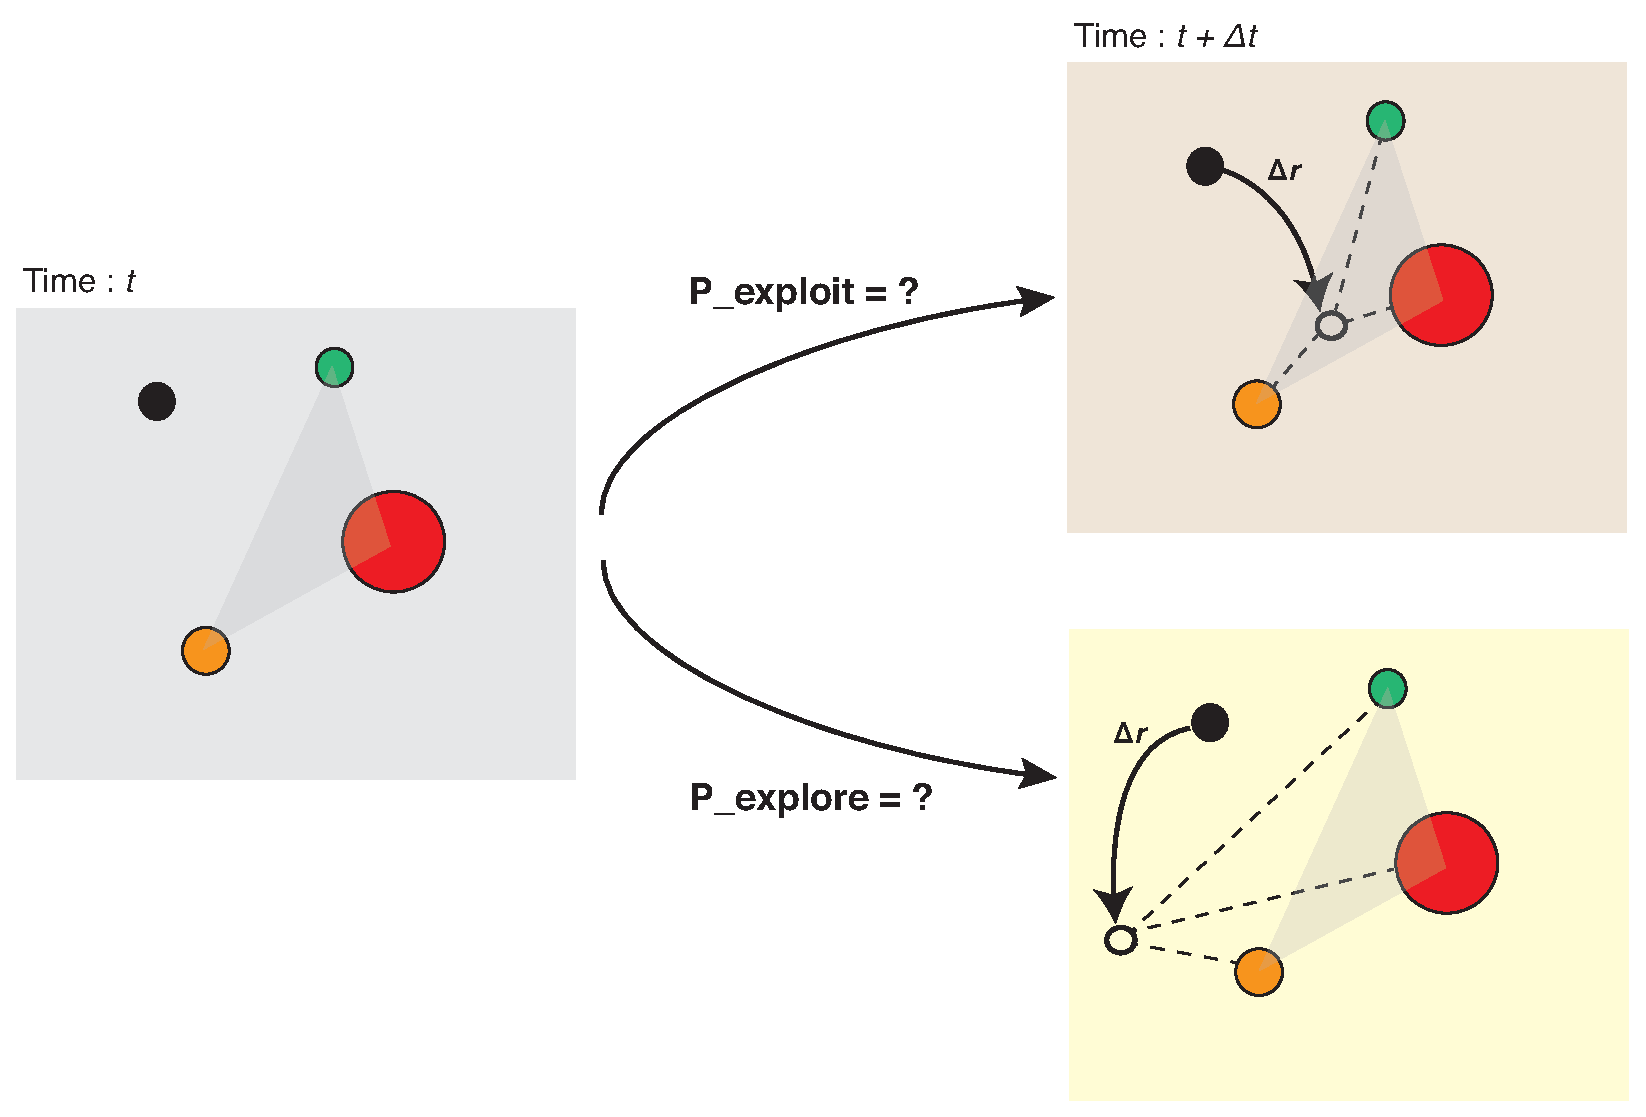
\includegraphics[width=10cm]{figures/schematic_displacement.eps}
\caption{\footnotesize{2-dimensional schematic description of the {\it L\'evy flying mind} model ({\bf ``Proportional Attraction"}): At each time step, the individual must choose between remaining in the solution envelope that has already been explored and exploring outside the currently known solution envelope.  We assign some probability $p$ (a number between 0 and 1) to the participant's decision of staying in the explored envelop and probability $1-p$ to the decision to explore outside that envelop.  If it is harder to find solutions that offer a balanced re-combination of previous solutions than to think out-of-the-box and propose solutions outside of the current solution envelope, then $p < \frac{1}{2}$ else $p \geq \frac{1}{2}$.}}
\label{fig:schematic}
\end{center}
\end{figure}

\section{What can we learn from stylised facts regarding timing ?}

\section{Discrete cascading models and recombination of knowledge}




\section{Discussion}

Outstanding problems :

- decreasing mean square displacement: it basically seems that with time displacement decreases: This can be due to (i) the limited space (unlikely), (ii) some convergence toward the true model, or (iii) some stickiness, or (iv) probably (ii) and (iii) together.
  
- connecting cascades and memory with (i) evolutionary theory and (ii) increased success (resp. counter-performance). Connect also with potential cascading processes in cognition (any knowledge about this? memory?)

- time between return visits (if return visits happen in close time, then it matters little)

- connect results with Distance Decay, but basically a model could be summarized as $Distance \sim S_T$ (by the way $D_{min}$ versus $S_T$ could be improved by looking at $D_t$ versus $S_t$). $S_T$ (resp. $S_t$) is a function of displacement $\Delta r$ decisions (which may also cost additional time) and (obviously) their influence on score. 

In summary, there is at some point a displacement decision with a part of ``risk", which can by the way be discounted by time spent (waiting time relative to avg waiting time and/or experimentation duration and/or time left). Large displacement can be associated with more risky exploration and more time required for decision. It looks like there is a $\Delta r$ which maximize improvement ($\Delta r \approx 0.15$). This is interesting because it suggests that such move size maximizes the chance that a new patch will be visited.


potential long reach :

- qualitative/quantitative differences between performing/non-performing participants?













\section{Conclusion}


\clearpage
%\section{The Experiment} 

Our data comes from an experiment which we conducted at Columbia University's Social Science laboratory.  Participants were given a graphical environment in which they could express their exact believes with respect to the causal structure and probabilistic relationships between 3 or 4 related binary variables, depending on treatment.  Participants were compensated according to their predictions and their predictions' congruence with a series of realizations.  Participants were enabled to dynamically update their models.   The incentives to make good predictions were determined according to an incentive scheme that is standard in experimental economics known as the Becker–DeGroot–Marschak method.  

\section{Experimental Design and Implementation}

\subsection{Causal Reasoning about a set of Binary Variables}

Here, we describe and informally define the kinds of systems that experimental participants reasoned about as they participated in our experiment on causal reasoning. 

\subsubsection{The noisy-or operator \citep{Pearl88}}

For systems with only binary variables we might think of causation in the following way as suggested by Judea Pearl in 1988.  If causation only involves 2 variables, say $A$ and $B$, where $A$ has a positive causal effect on $B$, then things are simple:

$P(B = 1 | A = 1) = p$, where $p \in [0, 1]$ and 0 otherwise.  That is, if the cause is present, $B=1$ follows with probability $p$, else it never happens, as there is only one possible cause for $B$ to assume the value $1$ and that is for $A$ to assume the value $1$. Note that in reverse this will mean $P(A=1|B=1)=1$. $B$ can only assume the value $1$ when $A$ is $1$ and thus observing that $B$ is $1$ tells us that $A$ must be $1$ as well. The cookies are gone and there was only one person here who could have eaten them! 

Other definitions have it that a causal effect of A on B is positive if $P(B = 1 | A = 1) > P(B = 1 | A = 0)$ and $P(B = 0 | A = 1) < P(B = 0 | A = 0)$, but that suggests that there are some ommitted causes of the event $B=1$. 

Keeping with Judea Pearl's 1986 reasoning, we ask how best to think about causation when there are two binary causes, $B$ and $C$ and one binary outcome. We then generalize this idea. 

The naive way to pose that would be as:

$P(A=1|B=b, C=c) = \pi_B*b + \pi_C*c$, 

where $b, c \in \{1, 0\}$ are the values taken on by the variables $B$ and $C$ and $\pi_B$, $\pi_C \in [0,1]$ are the causal effects of $B$ on $A$ and $C$ on $A$ respectively. But the problem with this formulation -- as Pearl pointed out -- is that, since $P(A=1|B=b, C=c)$ is a probability, as such it must take a value between $0$ and $1$.

The constraint $0< \pi_B*b + \pi_C*c <1$ induces a dependence between the causal effects $\pi_B$ and $\pi_C$ that we had not explicitly intended in our theory, which posed that $B$ and $C$ each independently cause $A$. Our implicit theory takes the following explicit form \citep{Pearl88}:

$P(A=1|B=b, C=c) = 1-(1-\pi_B)^b(1-\pi_C)^c$.

Pearl called it the noisy-OR operator because, supposing $\pi_B=\pi_C=1$, $A$ will be $1$ exactly whenever $B=1$, $C=1$, or both.  When $\pi_B, \pi_C \in (0, 1)$, the OR operator is noisy. The noisy-OR operator accommodates negative causation and any finite number of causes: 

$P(A=1|B=b, C=c, D=d) = 1-(1-\pi_B)^b(1-\pi_C)^{1-c}(1-\pi_D)^d$,

where the exponant, $1-c$ in the term $(1-\pi_C)^{1-c}$ means that the variable $C$ exerts a negative causal influence on the variable $A$.

For a set of binary variables, then, this simple system defines a causal grammar that allows us to construct almost arbitrary causal structures relating the members of the set.  The only constraint is that one may not propose a model with causal cycles. Such models are logically incoherent, unless we allow for dynamics which we don't in this experiment. Here we're going to restrict ourselves to cases where there are no dynamics, there is just a process that repeats in time, like the proverbial coin flip, but with more or less intricate (complex) internal structures.

\subsection{Experimental Treatments}

Data from such systems can also be simulated and presented to people so that they may backward engineer the causal structures that generated this data. That is, experimental participants see data and build causal models, seeking to understand how the data was produced and to make predictions of future observations. 

To make things more relatable, we labeled the variables with names from economics, as these seem to relate to many people: "Interest Rate (IR)", "Financial Sector (FS)", "industry (ID)" and "Consumer Spending (CS)". 

%As a side note, it would be interesting so see how labeling could affect learning and diversity.  It can for example be postulated and I find it likely that it is hard for certain people to learn certain relationships because of the meaning that is attached to labels.  Note that I did not include "Taxes" as a variable lable, as this label is a likely candidate to induce hard learning.    

We thus simulated from the joint distributions of two such systems, one simpler and the other more complex and presented people with the data and the modeling tools to try to learn the causal relationships and parameter values in these systems. The simpler system has three variables: "Interest Rate (IR)", "Financial Sector (FS)" and "Industry (ID)", where the "Interest Rate" has a negative effect on the "Industry" and the "Financial Sector" has a positive effect on the "Industry" (our somewhat arbitrary settings).

For the simple treatment, the data that the participants observed were generated in the following way: a variable was chosen at random from the system's variables to be the current period's "betting bariable". The value of this variable was hidden from the participants until the end of the period. Participants were incentivised to predict the value of this variable. Next, the value of the "interest Rate" variable was drawn; "H", with probability $0.5$ and "L: with probability $0.5$, followed by the value of the "Financial Sector" variable, with identical probabilities. Lastly, the value of the "Industry" variable was drawn, according to the conditional probability:  

$P(ID=1|FS=fs, IR=ir) = 1-(1-\pi_{FS})^{fs}(1-\pi_{IR})^{1-ir}$, where $\pi_{FS}=\pi_{IR}=0.5$. 

The more complex system had four variables labelled "Interest Rate (IR)", "Financial Sector (FS)", "Industry (ID)" and "Consumer Spending (CS)", where as before the "Interest Rate" has a negative effect on the "Industry" and the "Financial Sector" has a positive effect on the "Industry". In addition, in this system the "Industry" and "Interest Rate" also affect "Consumer Spending". "Industry" positively and the "Interest Rate" negatively.  Please do not hold us accountable for those choices, we will not defend these particular configurations in any way.

The joint distributions of Bayesian Belief Nets can be caculated as the products of the conditional probabilities and the marginal probabilities, as follows. For any number of related variables, $X_1, \ldots, X_n$, their joint probability can be calculated as:

$P(x_1, \ldots, x_n) = P(x_1 | x_2, \ldots, x_n)*P(x_2 | x_3, \ldots, x_n)*\cdots*P(x_{n-1} |x_n)*P(x_n)$.
\\

$P(x_1, \ldots, x_n) = P(x_1 | x_2, \ldots, x_n)*P(x_2 | x_3, \ldots, x_n)*\cdots*P(x_{n-1} |x_n)*P(x_n)$.
\\

For example, remembering that $P(ID=1|FS=fs, IR=ir) = 1-(1-\pi_{FS})^{fs}*(1-\pi_{IR})^{1-ir}$, where $\pi_{FS}=\pi_{IR}=0.5$, for the simple treatment, the joint outcome $FS=H, IR=H, ID=H$ has probability:
\\

$P(FS=H, IR=H, ID=H) = P(ID=1|FS=H, IR=H)*P(FS=H)*P(IR=H)=\left(1-(1-\pi_{FS})^{1}*(1-\pi_{IR})^{1-1}\right)*0.5^2 =0.125.$  
\\

A frequentist, might simply count membership of the joint buckets and build a model that matches the percentages. Updating her beliefs in this context of a repeating process, a bayesian could essentially do the same thing by comparing members of the dirichlet distribution class by obeserving, updating and finding the maximum of the posterior distribution of the parameters, known as the pseudo counts. This maximum turns out to approach the $2^k$ dimensional value of the bin counts. Likewise, all conditional distributions could be calculated in this way, but cognitive scientists and computer scientists have recently found this to be computationally more expensive than necessary \citep{Griffith08, Koller03}.  They suggest that instead of calculating $2^k$ parameters for the joint distribution of $k$ binary variables, people and computers should build structural models, where they can update their beliefs for a much reduced number of parameters and obtain the same results. For the model that we used as the simple treatment process, for example, if one has the right structure and the correct idea that $P(ID=1|FS=0, IR=1)=0$, there are four parameters to form beliefs about: $\pi_{FS}, \pi_{IR}, P(FS), P(IR)$. But perhaps, one doesn't see causation in that way and then there are $5$ parameters.  The full joint distribution has eight parameters.  There are thus less parameters to estimate if a causal theory is postulated. The benefit of thinking structurally will increase as the number of variables gets large because most often, the number of causal relationships (structural parameters) increases linearly in the number of variables, $k$, whereas the parameters of the joint distribution increases exactly by $2^k$.  At most, each variable that is added, affects every variable that is already there and then the number of causal arrows grows with $k$ as $k(1-k)$. In light of this, it seems evident that people should have a harder time guessing the correct structure and estimating the correct structural parameters when the system is complex than when it is simple. This should lead their models to be more diverse and less accurate in the complex case. 



\bibliographystyle{apsrev4-1}
\bibliography{bib/references,bib/cognition_causality,bib/L\'evyflight_foraging,bib/misc,bib/orgsci}

\clearpage
%\section{Experimental Design and Implementation}
\label{SI_experiment}

The data used in this work come from an experiment that we ran using an experimental platform 
designed to measure how participants form and update causal beliefs in more or less complex 
settings.  The experiment was conducted at Columbia University Social Science laboratory and 
involved 96 subjects.  Upon arrival, subjects were briefed and directed to an individual booth . 
The experiment was performed on a graphical  html/javascript interactive Web interface. All 
actions taken on the interface by subjects were recorded in real-time (resolution : $1s$). 

In the experiment, participants see a data stream: data about multiple binary variables in a 
system, which take on the value High or Low. For example, one variable could be a stock price 
and there may be a number of variables that explain its variation or are explained by its variation 
in turn.  A visual interface allows the subjects to draw a causal model of the system. The platform 
then computes predictions on the basis of the participant's causal model and makes those 
prediction visible to the participant. The participant then makes bets using these predictions. In 
doing so, the participant gets feedback on the accuracy of her beliefs, and can update her beliefs 
by modifying the causal model. The platform thus allows us to observe beliefs and learning in a 
very precise and controlled way.

\subsection{Experimental Treatments}
Data from probabilistic causal systems can be simulated and presented to people so that they may reverse engineer the causal 
structures that generated the patterns that they see. That is, experimental participants see data and build causal models, seeking to 
understand how the data was produced and to make predictions of future observations. \\

To make things concrete yet not obvious , we labeled the variables with names from economics, as these seem to relate to many 
people: "Interest Rate (IR)", "Financial Sector (FS)", "industry (ID)" and "Consumer Spending (CS)". We thus {\bf [simulated]} from the joint distributions of two such systems, one simpler and the other more complex and presented  people with the data and the modeling tools to learn the causal relationships and parameter values in these systems. The simpler system has three variables: "Interest Rate (IR)", "Financial Sector (FS)" and "Industry (ID)", where the "Interest Rate" has a negative effect on the "Industry" and the "Financial Sector" has a positive effect on the "Industry" (our somewhat arbitrary settings).\\

For the simple treatment, the data that the participants observed were generated in the following way: a variable was chosen at 
random from the system's variables to be the current period's "betting variable". The value of this variable was hidden from the 
participants until the end of the period. Participants were incentivised (on hand the well known Becker–DeGroot–Marschak 
method) to predict the value of this variable. Next, the value of the "interest Rate" variable was drawn; "H", with probability $0.5$ 
and "L: with probability $0.5$, followed by the value of the "Financial Sector" variable, with identical probabilities. Lastly, the value of 
the "Industry" variable was drawn according to Judea Pearl's \citep{Pearl88} probabilistic-OR operator, which gives the conditional 
probability:  

\be
P(ID=1|FS=fs, IR=ir) = 1-(1-\pi_{FS})^{fs}(1-\pi_{IR})^{1-ir} ~with ~ \pi_{FS} = \pi_{IR}=0.5
\ee

The more complex system had four variables labeled "Interest Rate (IR)", "Financial Sector (FS)", "Industry (ID)" and "Consumer 
Spending (CS)", where as before the "Interest Rate" has a negative effect on the "Industry" and the "Financial Sector" has a positive 
effect on the "Industry". In addition, in this system the "Industry" and "Interest Rate" also affect "Consumer Spending". "Industry" 
positively and the "Interest Rate" negatively.  Please do not hold us accountable for those choices, we will not defend these 
particular configurations in any way.

The joint distributions of Bayesian Belief Nets can be calculated as the products of the conditional probabilities and the marginal 
probabilities, as follows. For any number of related variables, $X_1, \ldots, X_n$, their joint probability can be calculated as:

\be
P(x_1, \ldots, x_n) = P(x_1 | x_2, \ldots, x_n) \times P(x_2 | x_3, \ldots, x_n) \times \cdots \times P(x_{n-1} |x_n) \times P(x_n).
\ee

For example, remembering that $P(ID=1|FS=fs, IR=ir) = 1-(1-\pi_{FS})^{fs} \times (1-\pi_{IR})^{1-ir}$, where $\pi_{FS}=\pi_{IR}=0.5$, for 
the simple treatment, the joint outcome $FS=H, IR=H, ID=H$ has probability:\\

\ba
P(FS=H, IR=H, ID=H) =\\ 
P(ID=1|FS=H, IR=H) \times P(FS=H) \times P(IR=H) \\
=  \left(1-(1-\pi_{FS})^{1} \times (1-\pi_{IR})^{1-1}\right) \times 0.5^2 =0.125.  
\ea

A frequentist, might simply count membership of the joint buckets and build a model that matches the percentages. Updating her beliefs in this context of a repeating process, a Bayesian could essentially do the same thing by comparing members of the Dirichlet distribution class (for example, depending on priors) by observing, updating and finding the maximum of the posterior distribution of the parameters, known as the pseudo counts. This maximum turns out to approach the $2^k$ dimensional value of the bin counts. Likewise, all conditional distributions could be calculated in this way, but cognitive scientists and computer scientists have recently found this to be computationally more expensive than necessary \citep{Griffith08, Koller03}.  They suggest that instead of calculating $2^k$ parameters for the joint distribution of $k$ binary variables, people and computers should build structural models, where they can update their beliefs for a much reduced number of parameters and obtain the same results. For the model that we used as the simple treatment process, for example, if one has the right structure and the correct idea that $P(ID=1|FS=0, IR=1)=0$, there are four parameters to form beliefs about: $\pi_{FS}, \pi_{IR}, P(FS), P(IR)$. But perhaps, one doesn't see causation in that way and then there are $5$ parameters.  The full joint distribution has eight parameters.  There are thus less parameters to estimate if a causal theory is postulated. The benefit of thinking structurally will increase as the number of variables gets large because most often, the number of causal relationships (structural parameters) increases linearly in the number of variables, $k$, whereas the parameters of the joint distribution increases exactly by $2^k$.  At most, each variable that is added, affects every variable that is already there and then the number of causal arrows grows with $k$ as $k(1-k)$. In light of this, it seems evident that people should have a harder time guessing the correct structure and estimating the correct structural parameters when the system is complex than when it is simple. This, we hypothesized, should lead their models to be more diverse and less accurate in the complex case. 

%\subsection{Causal Reasoning about a set of Binary Variables}

%Here, we describe and informally define the kinds of systems that experimental participants reasoned about as they participated in our experiment on causal reasoning. 

%\subsubsection{The noisy-or operator \citep{Pearl88}}

%For systems with only binary variables we might think of causation in the following way as suggested by Judea Pearl in 1988.  If causation only involves 2 variables, say $A$ and $B$, where $A$ has a positive causal effect on $B$, then things are simple:

%$P(B = 1 | A = 1) = p$, where $p \in [0, 1]$ and 0 otherwise.  That is, if the cause is present, $B=1$ follows with probability $p$, else it never happens, as there is only one possible cause for $B$ to assume the value $1$ and that is for $A$ to assume the value $1$. Note that in reverse this will mean $P(A=1|B=1)=1$. $B$ can only assume the value $1$ when $A$ is $1$ and thus observing that $B$ is $1$ tells us that $A$ must be $1$ as well. The cookies are gone and there was only one person here who could have eaten them! 

%Other definitions have it that a causal effect of A on B is positive if $P(B = 1 | A = 1) > P(B = 1 | A = 0)$ and $P(B = 0 | A = 1) < P(B = 0 | A = 0)$, but that suggests that there are some ommitted causes of the event $B=1$. 

%Keeping with Judea Pearl's 1986 reasoning, we ask how best to think about causation when there are two binary causes, $B$ and $C$ and one binary outcome. We then generalize this idea. 

%The naive way to pose that would be as:

%$P(A=1|B=b, C=c) = \pi_B \times b + \pi_C \times c$, 

%where $b, c \in \{1, 0\}$ are the values taken on by the variables $B$ and $C$ and $\pi_B$, $\pi_C \in [0,1]$ are the causal effects of $B$ on $A$ and $C$ on $A$ respectively. But the problem with this formulation -- as Pearl pointed out -- is that, since $P(A=1|B=b, C=c)$ is a probability, as such it must take a value between $0$ and $1$.

%The constraint $0< \pi_B \times b + \pi_C \times c <1$ induces a dependence between the causal effects $\pi_B$ and $\pi_C$ that we had not explicitly intended in our theory, which posed that $B$ and $C$ each independently cause $A$. Our implicit theory takes the following explicit form \citep{Pearl88}:

%$P(A=1|B=b, C=c) = 1-(1-\pi_B)^b(1-\pi_C)^c$.

%Pearl called it the noisy-OR operator because, supposing $\pi_B=\pi_C=1$, $A$ will be $1$ exactly whenever $B=1$, $C=1$, or both.  When $\pi_B, \pi_C \in (0, 1)$, the OR operator is noisy. The noisy-OR operator accommodates negative causation and any finite number of causes: 

%$P(A=1|B=b, C=c, D=d) = 1-(1-\pi_B)^b(1-\pi_C)^{1-c}(1-\pi_D)^d$,

%where the exponant, $1-c$ in the term $(1-\pi_C)^{1-c}$ means that the variable $C$ exerts a negative causal influence on the variable $A$.

%For a set of binary variables, then, this simple system defines a causal grammar that allows us to construct almost arbitrary causal structures relating the members of the set.  The only constraint is that one may not propose a model with causal cycles. Such models are logically incoherent, unless we allow for dynamics which we don't in this experiment. Here we're going to restrict ourselves to cases where there are no dynamics, there is just a process that repeats in time, like the proverbial coin flip, but with more or less intricate (complex) internal structures.



%As a side note, it would be interesting so see how labeling could affect learning and diversity.  It can for example be postulated and I find it likely that it is hard for certain people to learn certain relationships because of the meaning that is attached to labels.  Note that I did not include "Taxes" as a variable lable, as this label is a likely candidate to induce hard learning.    






\section{Experiment}
\label{si:experiment}

\section{Jump Sizes $\Delta r$}

Euclidean distance : 

\begin{equation}
\Delta r = d(p, q) = \sqrt{(p_1- q_1)^2 + (p_2 - q_2)^2+\cdots+(p_i - q_i)^2+\cdots+(p_n - q_n)^2}.
\end{equation}

with $n=8$ (3-nodes BayesNet) or $n=16$ (4-npdes BayesNet) and $p$,$q$, 2 consecutive position vectors

\begin{figure}[h!]
\begin{center}
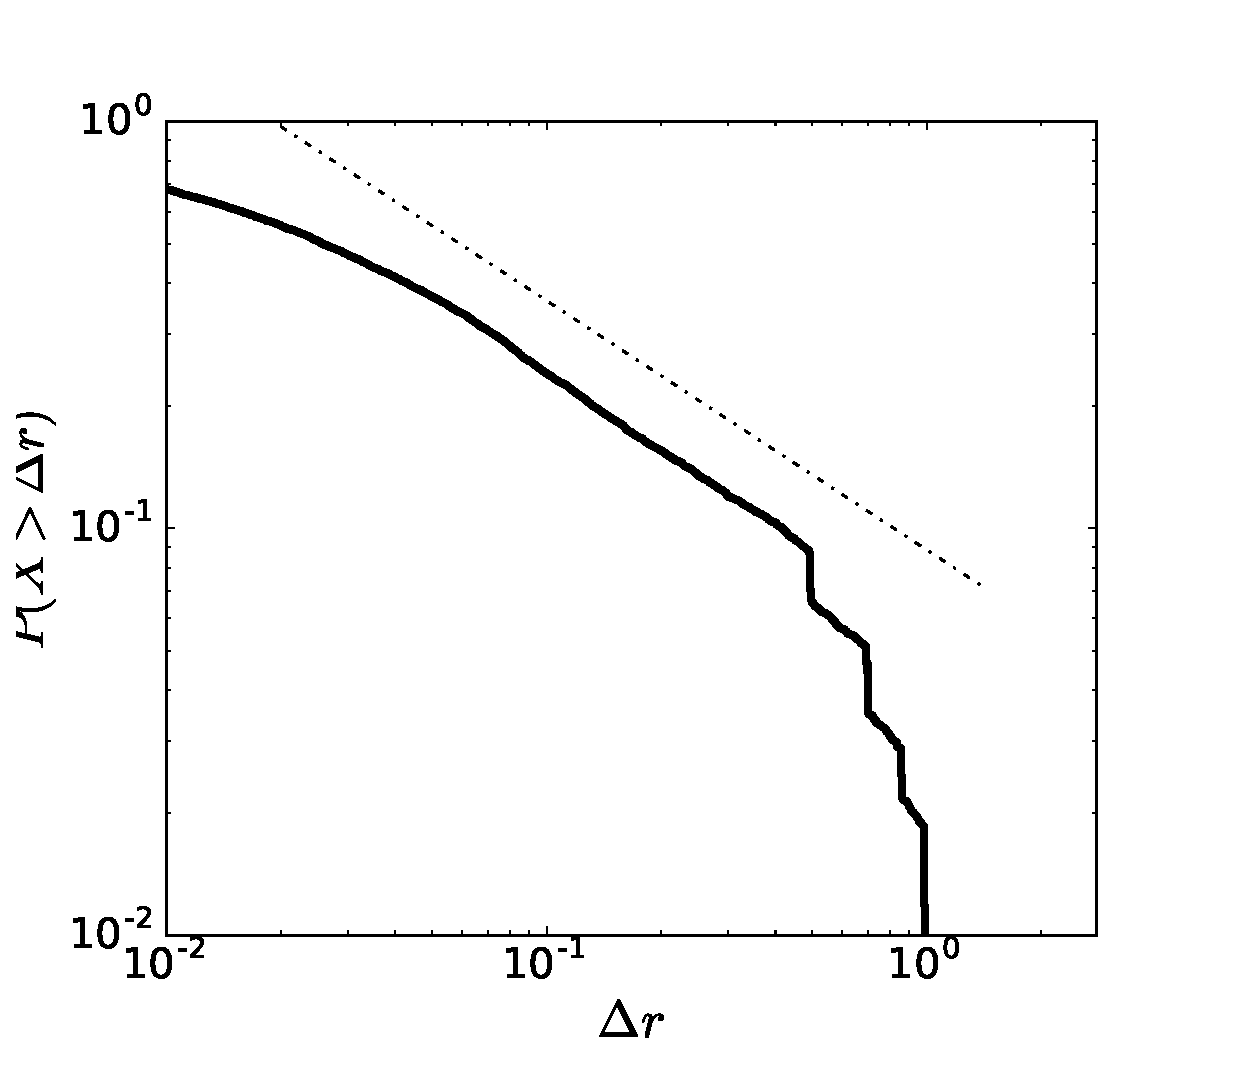
\includegraphics[width=10cm]{figures/CCDF_Displacement_simple.eps}
\caption{(3-node BayesNet) : exponent $\alpha = 0.61(3)$ with upper cutoff  $x_{max} \approx 1.4$ (theoretical limit is $x_{max} = 2\sqrt{2}$).}
\label{fig:jump_sizes}
\end{center}
\end{figure}


\section{Waiting Times $\Delta t$}



\begin{figure}[h!]
\begin{center}
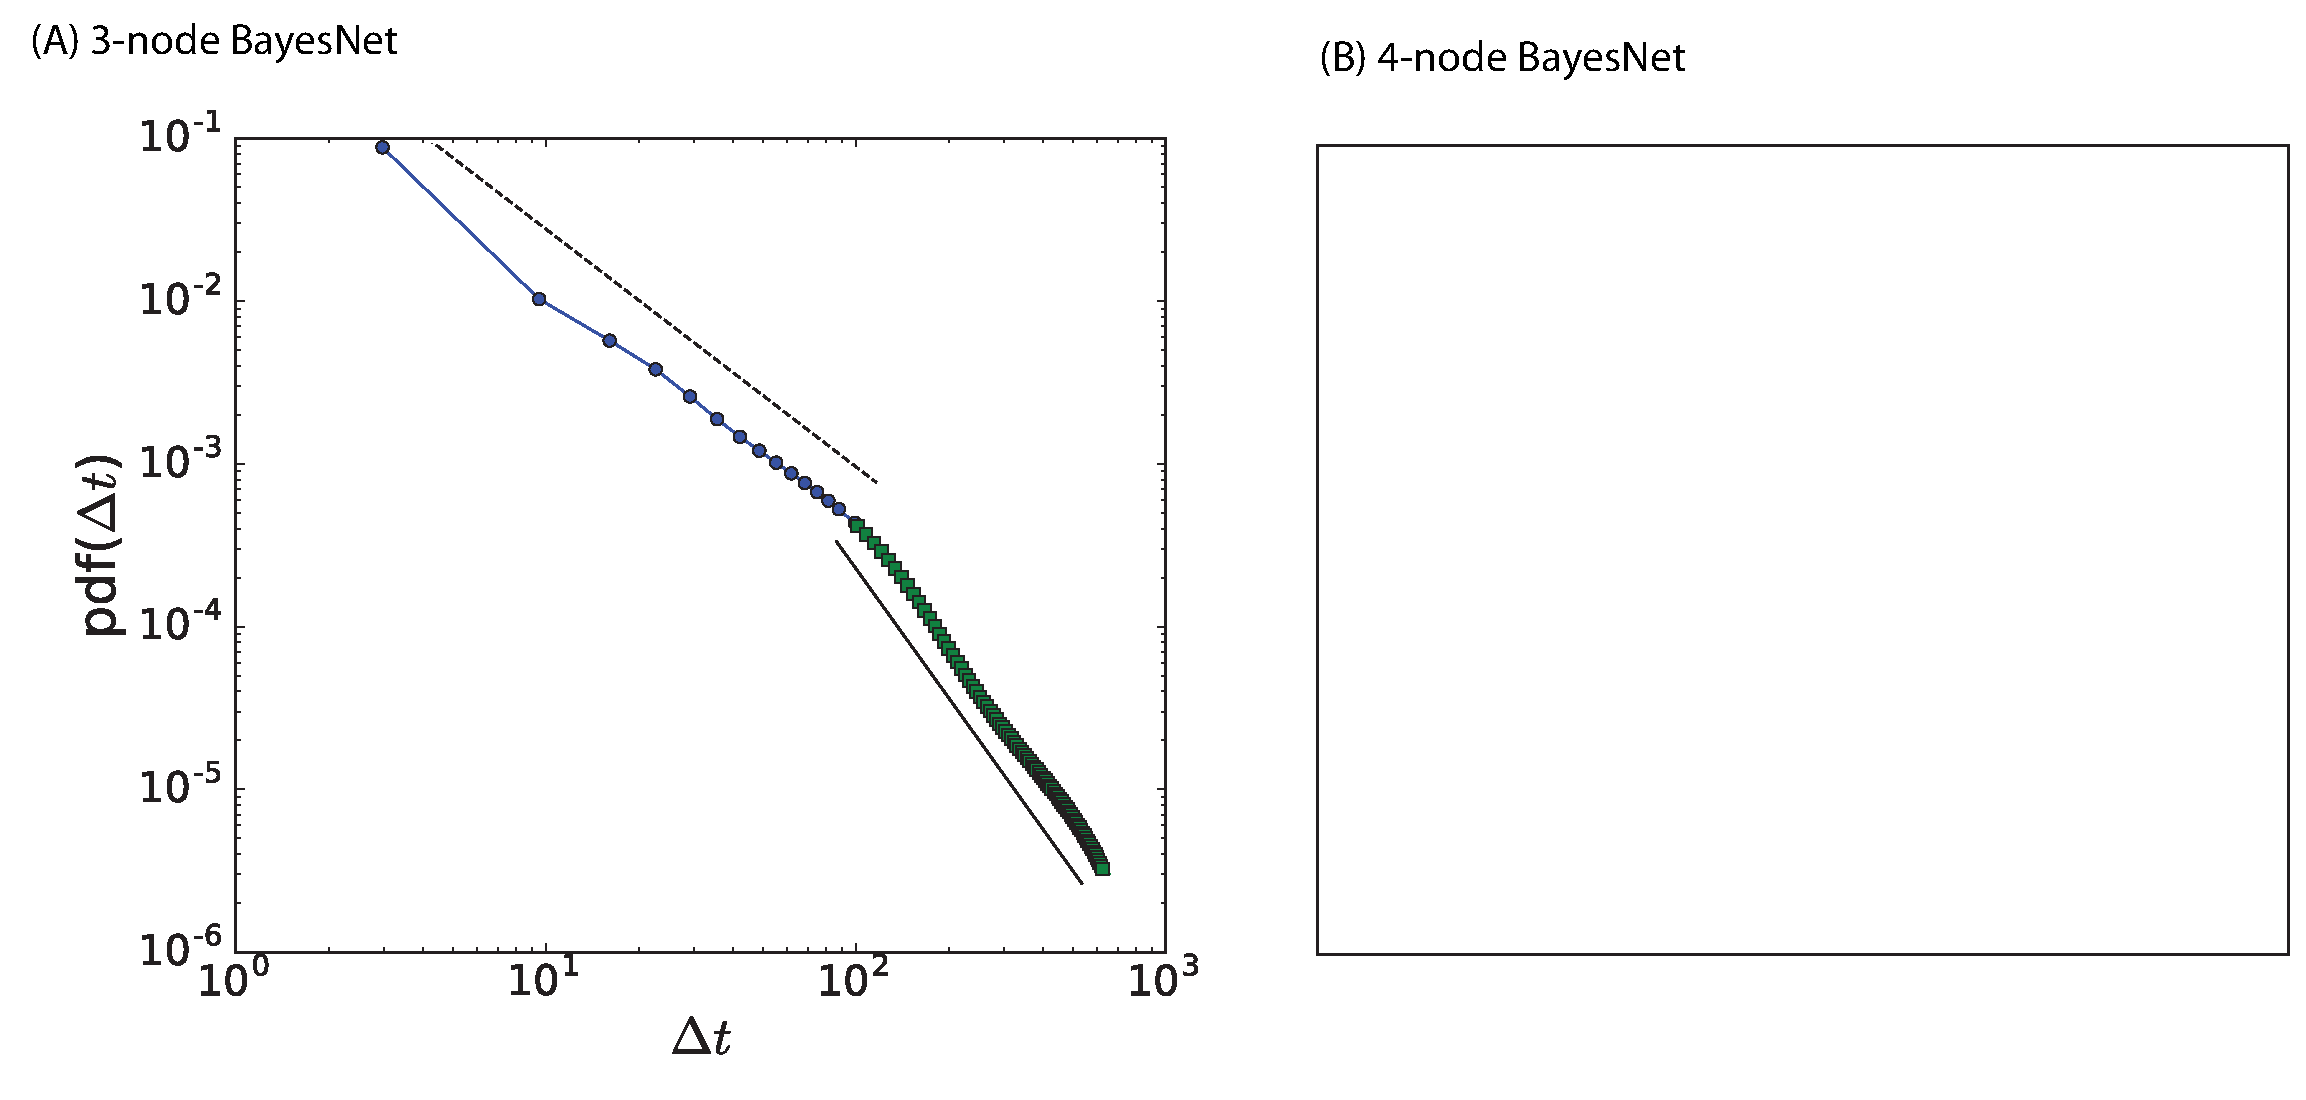
\includegraphics[width=15cm]{figures/dt_kernel_SI.eps}
\caption{Distribution of Waiting Times (fitted by kernel density estimators \cite{}) exhibits a change of regime typical of changes of regimes in waiting times \cite{maillart2011,saichevTheory}: $\beta_{\Delta t  \leqslant 100} \approx 0.46(3)$ (slope $\sim t^{-(1+ \beta_{\Delta t  \leqslant 100})}$ represented by dashed line) and $\beta_{\Delta t > 100} \approx 1.65(1)$ (slope $\sim t^{-(1+ \beta_{\Delta t  > 100})}$ represented by continuous line).}
\label{fig:waiting_times}
\end{center}
\end{figure}


\section{Correlation $\Delta r$ and $\Delta t$}
\label{si:corr_dr_dt}


\begin{figure}[h!]
\begin{center}
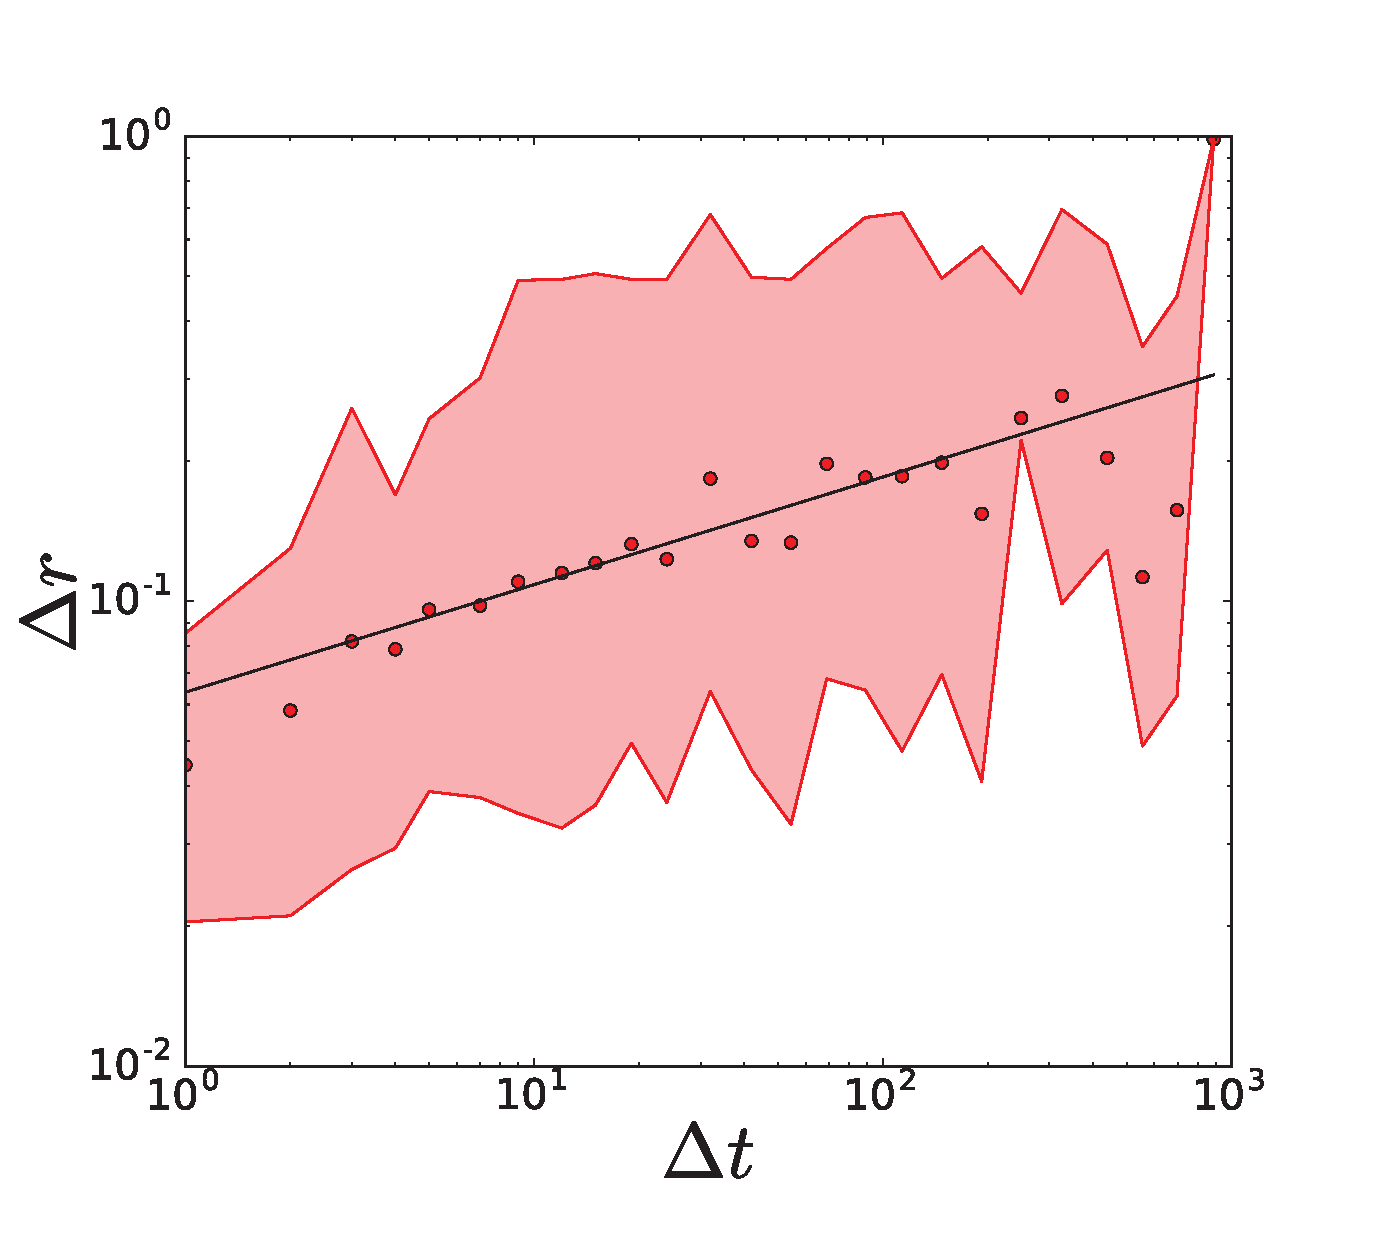
\includegraphics[width=10cm]{figures/cor_Delta_t_Delta_r_simple.eps}
\caption{3-node BayesNet : Correlation (Spearman rank correlation) between $corr(\Delta r,\Delta t) \approx 0.32$, and the main direction of dependence can be approximated by a scaling function $\Delta r \sim {(\Delta t)}^{0.23(2)}$ (least square fit of values in double logarithmique scale, $p < 0.001$ and $R= 0.21$}
\label{fig:corr_dr_dt}
\end{center}
\end{figure}






%\renewcommand\thesection{\Alph{section}}
\renewcommand\thesection{S\arabic{section}}
\setcounter{section}{0}

\renewcommand\theequation{S\arabic{equation}}
\setcounter{equation}{0}


%\begin{center}
%{\Large Supplementary Information}
%\vspace{3 cm}
%\end{center}

%\section{Experimental Design and Implementation}
\label{SI_experiment}

The data used in this work come from an experiment that we ran using an experimental platform 
designed to measure how participants form and update causal beliefs in more or less complex 
settings.  The experiment was conducted at Columbia University Social Science laboratory and 
involved 96 subjects.  Upon arrival, subjects were briefed and directed to an individual booth . 
The experiment was performed on a graphical  html/javascript interactive Web interface. All 
actions taken on the interface by subjects were recorded in real-time (resolution : $1s$). 

In the experiment, participants see a data stream: data about multiple binary variables in a 
system, which take on the value High or Low. For example, one variable could be a stock price 
and there may be a number of variables that explain its variation or are explained by its variation 
in turn.  A visual interface allows the subjects to draw a causal model of the system. The platform 
then computes predictions on the basis of the participant's causal model and makes those 
prediction visible to the participant. The participant then makes bets using these predictions. In 
doing so, the participant gets feedback on the accuracy of her beliefs, and can update her beliefs 
by modifying the causal model. The platform thus allows us to observe beliefs and learning in a 
very precise and controlled way.

\subsection{Experimental Treatments}
Data from probabilistic causal systems can be simulated and presented to people so that they may reverse engineer the causal 
structures that generated the patterns that they see. That is, experimental participants see data and build causal models, seeking to 
understand how the data was produced and to make predictions of future observations. \\

To make things concrete yet not obvious , we labeled the variables with names from economics, as these seem to relate to many 
people: "Interest Rate (IR)", "Financial Sector (FS)", "industry (ID)" and "Consumer Spending (CS)". We thus {\bf [simulated]} from the joint distributions of two such systems, one simpler and the other more complex and presented  people with the data and the modeling tools to learn the causal relationships and parameter values in these systems. The simpler system has three variables: "Interest Rate (IR)", "Financial Sector (FS)" and "Industry (ID)", where the "Interest Rate" has a negative effect on the "Industry" and the "Financial Sector" has a positive effect on the "Industry" (our somewhat arbitrary settings).\\

For the simple treatment, the data that the participants observed were generated in the following way: a variable was chosen at 
random from the system's variables to be the current period's "betting variable". The value of this variable was hidden from the 
participants until the end of the period. Participants were incentivised (on hand the well known Becker–DeGroot–Marschak 
method) to predict the value of this variable. Next, the value of the "interest Rate" variable was drawn; "H", with probability $0.5$ 
and "L: with probability $0.5$, followed by the value of the "Financial Sector" variable, with identical probabilities. Lastly, the value of 
the "Industry" variable was drawn according to Judea Pearl's \citep{Pearl88} probabilistic-OR operator, which gives the conditional 
probability:  

\be
P(ID=1|FS=fs, IR=ir) = 1-(1-\pi_{FS})^{fs}(1-\pi_{IR})^{1-ir} ~with ~ \pi_{FS} = \pi_{IR}=0.5
\ee

The more complex system had four variables labeled "Interest Rate (IR)", "Financial Sector (FS)", "Industry (ID)" and "Consumer 
Spending (CS)", where as before the "Interest Rate" has a negative effect on the "Industry" and the "Financial Sector" has a positive 
effect on the "Industry". In addition, in this system the "Industry" and "Interest Rate" also affect "Consumer Spending". "Industry" 
positively and the "Interest Rate" negatively.  Please do not hold us accountable for those choices, we will not defend these 
particular configurations in any way.

The joint distributions of Bayesian Belief Nets can be calculated as the products of the conditional probabilities and the marginal 
probabilities, as follows. For any number of related variables, $X_1, \ldots, X_n$, their joint probability can be calculated as:

\be
P(x_1, \ldots, x_n) = P(x_1 | x_2, \ldots, x_n) \times P(x_2 | x_3, \ldots, x_n) \times \cdots \times P(x_{n-1} |x_n) \times P(x_n).
\ee

For example, remembering that $P(ID=1|FS=fs, IR=ir) = 1-(1-\pi_{FS})^{fs} \times (1-\pi_{IR})^{1-ir}$, where $\pi_{FS}=\pi_{IR}=0.5$, for 
the simple treatment, the joint outcome $FS=H, IR=H, ID=H$ has probability:\\

\ba
P(FS=H, IR=H, ID=H) =\\ 
P(ID=1|FS=H, IR=H) \times P(FS=H) \times P(IR=H) \\
=  \left(1-(1-\pi_{FS})^{1} \times (1-\pi_{IR})^{1-1}\right) \times 0.5^2 =0.125.  
\ea

A frequentist, might simply count membership of the joint buckets and build a model that matches the percentages. Updating her beliefs in this context of a repeating process, a Bayesian could essentially do the same thing by comparing members of the Dirichlet distribution class (for example, depending on priors) by observing, updating and finding the maximum of the posterior distribution of the parameters, known as the pseudo counts. This maximum turns out to approach the $2^k$ dimensional value of the bin counts. Likewise, all conditional distributions could be calculated in this way, but cognitive scientists and computer scientists have recently found this to be computationally more expensive than necessary \citep{Griffith08, Koller03}.  They suggest that instead of calculating $2^k$ parameters for the joint distribution of $k$ binary variables, people and computers should build structural models, where they can update their beliefs for a much reduced number of parameters and obtain the same results. For the model that we used as the simple treatment process, for example, if one has the right structure and the correct idea that $P(ID=1|FS=0, IR=1)=0$, there are four parameters to form beliefs about: $\pi_{FS}, \pi_{IR}, P(FS), P(IR)$. But perhaps, one doesn't see causation in that way and then there are $5$ parameters.  The full joint distribution has eight parameters.  There are thus less parameters to estimate if a causal theory is postulated. The benefit of thinking structurally will increase as the number of variables gets large because most often, the number of causal relationships (structural parameters) increases linearly in the number of variables, $k$, whereas the parameters of the joint distribution increases exactly by $2^k$.  At most, each variable that is added, affects every variable that is already there and then the number of causal arrows grows with $k$ as $k(1-k)$. In light of this, it seems evident that people should have a harder time guessing the correct structure and estimating the correct structural parameters when the system is complex than when it is simple. This, we hypothesized, should lead their models to be more diverse and less accurate in the complex case. 

%\subsection{Causal Reasoning about a set of Binary Variables}

%Here, we describe and informally define the kinds of systems that experimental participants reasoned about as they participated in our experiment on causal reasoning. 

%\subsubsection{The noisy-or operator \citep{Pearl88}}

%For systems with only binary variables we might think of causation in the following way as suggested by Judea Pearl in 1988.  If causation only involves 2 variables, say $A$ and $B$, where $A$ has a positive causal effect on $B$, then things are simple:

%$P(B = 1 | A = 1) = p$, where $p \in [0, 1]$ and 0 otherwise.  That is, if the cause is present, $B=1$ follows with probability $p$, else it never happens, as there is only one possible cause for $B$ to assume the value $1$ and that is for $A$ to assume the value $1$. Note that in reverse this will mean $P(A=1|B=1)=1$. $B$ can only assume the value $1$ when $A$ is $1$ and thus observing that $B$ is $1$ tells us that $A$ must be $1$ as well. The cookies are gone and there was only one person here who could have eaten them! 

%Other definitions have it that a causal effect of A on B is positive if $P(B = 1 | A = 1) > P(B = 1 | A = 0)$ and $P(B = 0 | A = 1) < P(B = 0 | A = 0)$, but that suggests that there are some ommitted causes of the event $B=1$. 

%Keeping with Judea Pearl's 1986 reasoning, we ask how best to think about causation when there are two binary causes, $B$ and $C$ and one binary outcome. We then generalize this idea. 

%The naive way to pose that would be as:

%$P(A=1|B=b, C=c) = \pi_B \times b + \pi_C \times c$, 

%where $b, c \in \{1, 0\}$ are the values taken on by the variables $B$ and $C$ and $\pi_B$, $\pi_C \in [0,1]$ are the causal effects of $B$ on $A$ and $C$ on $A$ respectively. But the problem with this formulation -- as Pearl pointed out -- is that, since $P(A=1|B=b, C=c)$ is a probability, as such it must take a value between $0$ and $1$.

%The constraint $0< \pi_B \times b + \pi_C \times c <1$ induces a dependence between the causal effects $\pi_B$ and $\pi_C$ that we had not explicitly intended in our theory, which posed that $B$ and $C$ each independently cause $A$. Our implicit theory takes the following explicit form \citep{Pearl88}:

%$P(A=1|B=b, C=c) = 1-(1-\pi_B)^b(1-\pi_C)^c$.

%Pearl called it the noisy-OR operator because, supposing $\pi_B=\pi_C=1$, $A$ will be $1$ exactly whenever $B=1$, $C=1$, or both.  When $\pi_B, \pi_C \in (0, 1)$, the OR operator is noisy. The noisy-OR operator accommodates negative causation and any finite number of causes: 

%$P(A=1|B=b, C=c, D=d) = 1-(1-\pi_B)^b(1-\pi_C)^{1-c}(1-\pi_D)^d$,

%where the exponant, $1-c$ in the term $(1-\pi_C)^{1-c}$ means that the variable $C$ exerts a negative causal influence on the variable $A$.

%For a set of binary variables, then, this simple system defines a causal grammar that allows us to construct almost arbitrary causal structures relating the members of the set.  The only constraint is that one may not propose a model with causal cycles. Such models are logically incoherent, unless we allow for dynamics which we don't in this experiment. Here we're going to restrict ourselves to cases where there are no dynamics, there is just a process that repeats in time, like the proverbial coin flip, but with more or less intricate (complex) internal structures.



%As a side note, it would be interesting so see how labeling could affect learning and diversity.  It can for example be postulated and I find it likely that it is hard for certain people to learn certain relationships because of the meaning that is attached to labels.  Note that I did not include "Taxes" as a variable lable, as this label is a likely candidate to induce hard learning.    






\section{Experiment}
\label{si:experiment}

\section{Jump Sizes $\Delta r$}

Euclidean distance : 

\begin{equation}
\Delta r = d(p, q) = \sqrt{(p_1- q_1)^2 + (p_2 - q_2)^2+\cdots+(p_i - q_i)^2+\cdots+(p_n - q_n)^2}.
\end{equation}

with $n=8$ (3-nodes BayesNet) or $n=16$ (4-npdes BayesNet) and $p$,$q$, 2 consecutive position vectors

\begin{figure}[h!]
\begin{center}
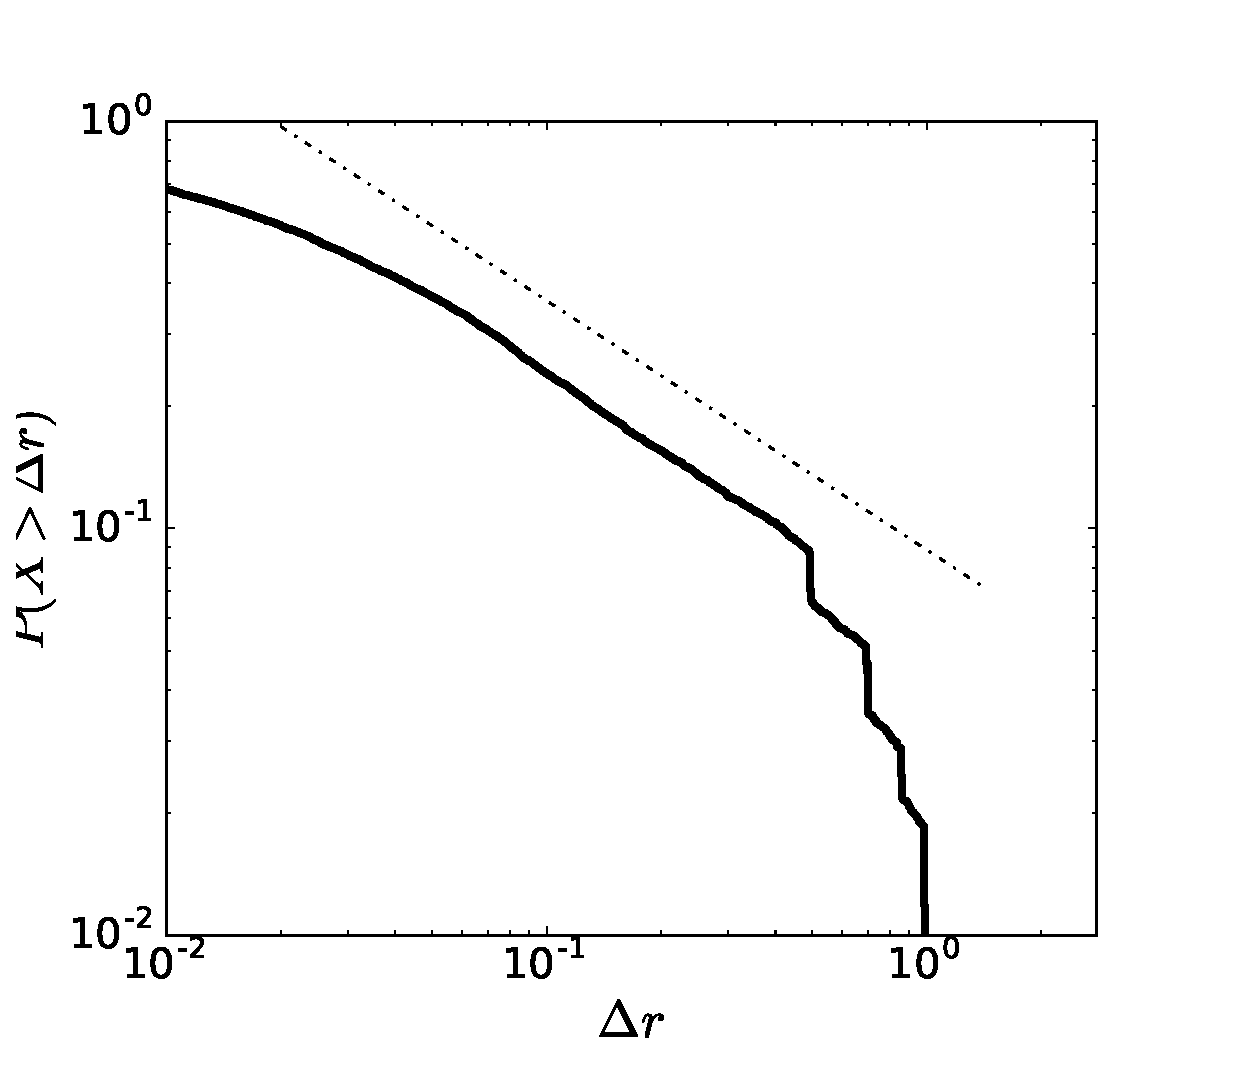
\includegraphics[width=10cm]{figures/CCDF_Displacement_simple.eps}
\caption{(3-node BayesNet) : exponent $\alpha = 0.61(3)$ with upper cutoff  $x_{max} \approx 1.4$ (theoretical limit is $x_{max} = 2\sqrt{2}$).}
\label{fig:jump_sizes}
\end{center}
\end{figure}


\section{Waiting Times $\Delta t$}



\begin{figure}[h!]
\begin{center}
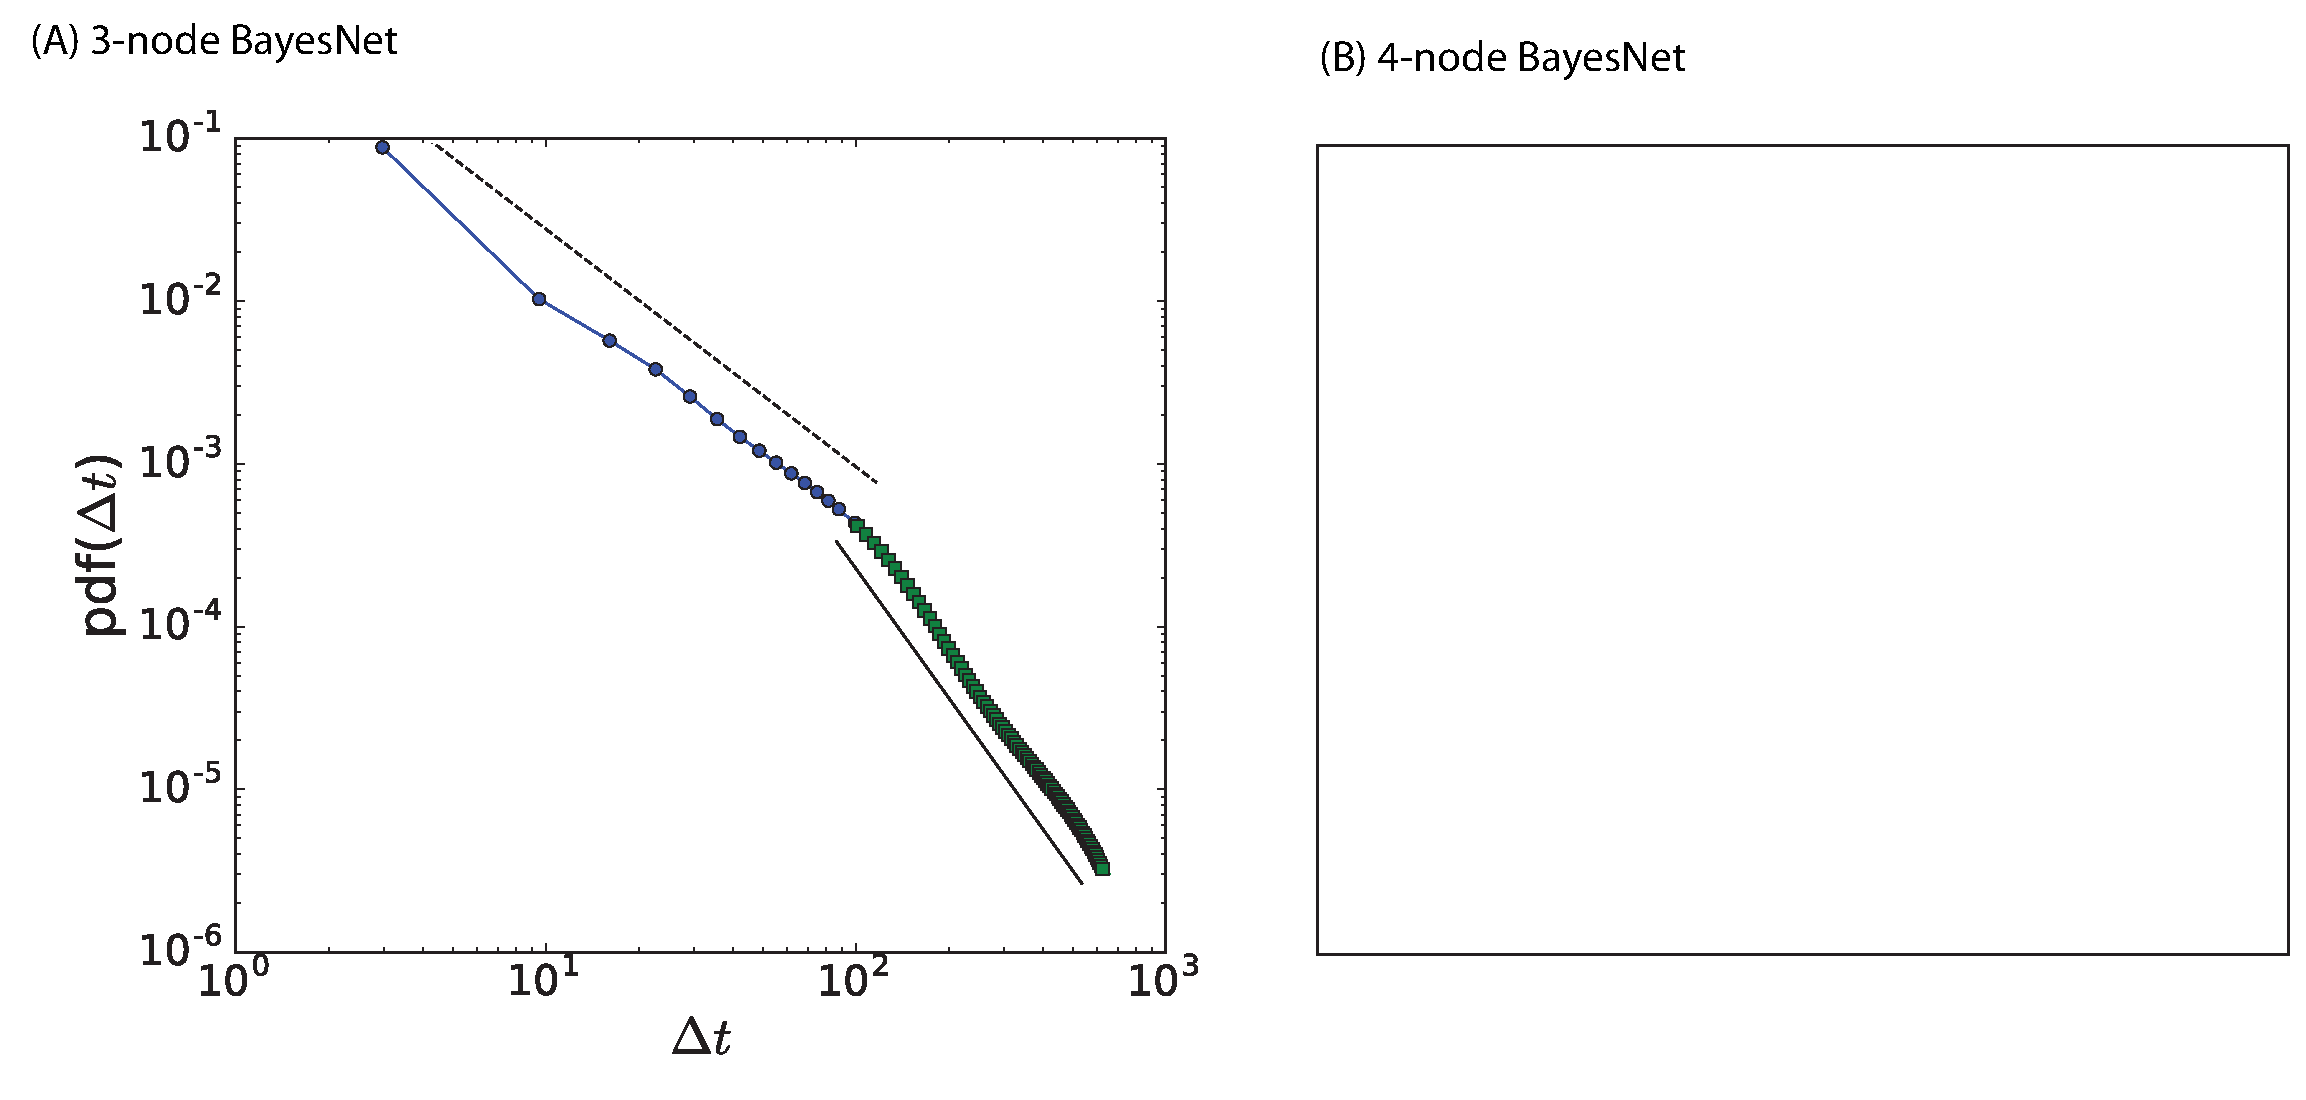
\includegraphics[width=15cm]{figures/dt_kernel_SI.eps}
\caption{Distribution of Waiting Times (fitted by kernel density estimators \cite{}) exhibits a change of regime typical of changes of regimes in waiting times \cite{maillart2011,saichevTheory}: $\beta_{\Delta t  \leqslant 100} \approx 0.46(3)$ (slope $\sim t^{-(1+ \beta_{\Delta t  \leqslant 100})}$ represented by dashed line) and $\beta_{\Delta t > 100} \approx 1.65(1)$ (slope $\sim t^{-(1+ \beta_{\Delta t  > 100})}$ represented by continuous line).}
\label{fig:waiting_times}
\end{center}
\end{figure}


\section{Correlation $\Delta r$ and $\Delta t$}
\label{si:corr_dr_dt}


\begin{figure}[h!]
\begin{center}
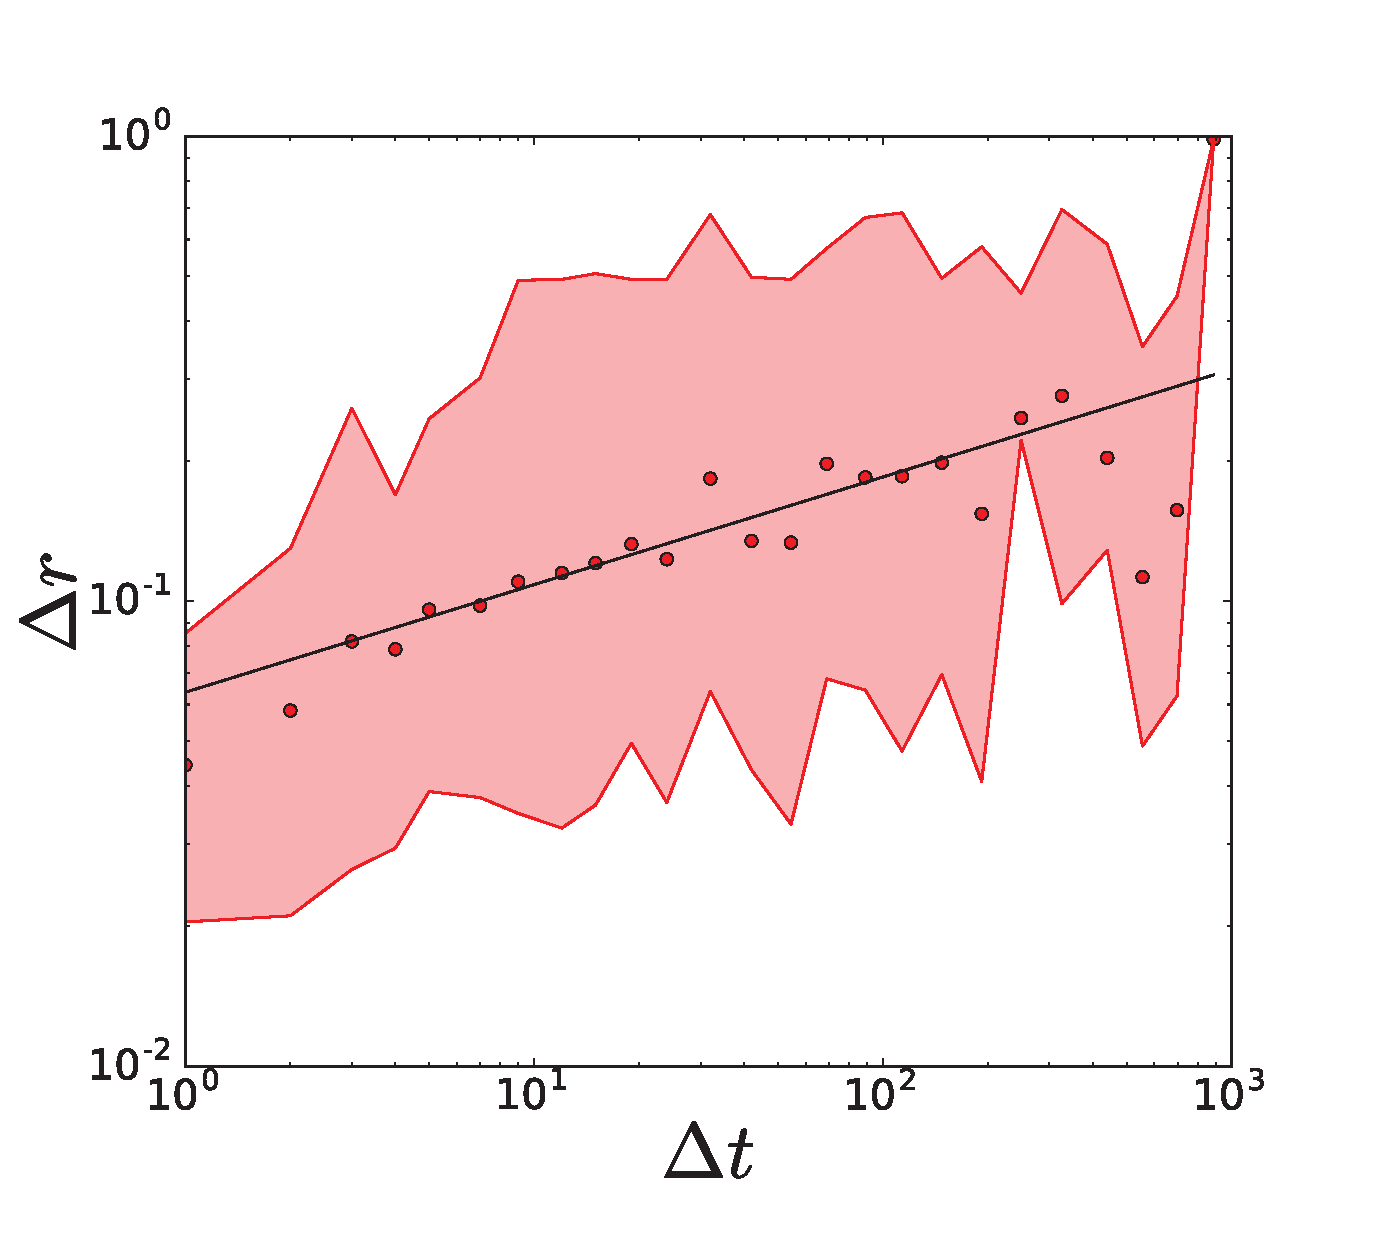
\includegraphics[width=10cm]{figures/cor_Delta_t_Delta_r_simple.eps}
\caption{3-node BayesNet : Correlation (Spearman rank correlation) between $corr(\Delta r,\Delta t) \approx 0.32$, and the main direction of dependence can be approximated by a scaling function $\Delta r \sim {(\Delta t)}^{0.23(2)}$ (least square fit of values in double logarithmique scale, $p < 0.001$ and $R= 0.21$}
\label{fig:corr_dr_dt}
\end{center}
\end{figure}





%\section{Literature Review}
The cognitive science and economics literatures have found much evidence in support of consistency with as well as deviance from human learning with Bayesian constructs of learning. On average, especially when incentives are higher or tasks simple, subjects update their beliefs based on new data in a way that is consistent with Bayes rule. However, at the individual level, there are large variations, as well as systematic departures under certain conditions.  In these literatures, comparing human learning to Bayesian updating, observed deviations can be organized in terms of "biases" or "heuristics".  Deterministic bias may have the consequence of underweighting or overweighting evidence ('law of small numbers' ) relative to base rates.  Such biases are in turn explained by the concept of availability heuristic (Griffin and Tversky 1992), which reduces data to examples that immediately come to mind, rather than by considering the exhaustive data of all previous experience and it has the consequence of slowing learning.  An example of the latter is recency bias (FudenbergPeysakhovich2014).  Another obstacle to efficient learning is when ambiguous information is taken to be a confirmation of a currently held hypothesis, or when information is suboptimally acquired or remembered.  Additionally, people have been found having difficulties with contingent reasoning with regards to future events (CharnessLevin2009). 
 
A different literature, associated with many disparate disciplines, such as ecology, cognitive science and complex systems frames learning and behavior in uncertain environments in terms of search, a ubiquitous property of life (Hills, Thomas T. et al. 2015).  Search, in turn, is a process of exploration and exploitation.  If behavior remains stable over some period of time, is focused and stays within a narrow subspace of the feasible decision or belief space it is interpreted as exploitation.  If it is erratic and moves wildly, it is interpreted as exploration (Mehlhorn et al, 2015).   

%These departures are clues to the heuristics humans use in their judgments, which overall often approximate bayesian inference but are not equivalent. Although many of these deviations imply that learning should be slower than predicted by Bayes rule,  few experiments measure the rate of learning and how far it departs from Bayesian inference.  

But why should one search and not simply count past events as Bayesian and Frequentist rationality demand (co-occurrences of values of a set of variables)?  With regards to counting observed frequencies of co-occurrences in order to measure covariances between a set of variables, if the number of variables gets large, the number of possible co-occurrences becomes astronomical.  Thus, remembering how many times a particular constellation of values of a given set of variables co-occurred puts ever increasing demands on memory as the set of variables gets large.  "In any system responsible for managing a vast data base there must be failures of retrieval" (Anderson, J. R., & Schooler, L. J. 1991).  Hence optimality must not mean Bayesian or Frequentist optimality, as counting all possible co-occurrences is not feasible because of limits on memory.  Additionally, there is the problem of assigning beliefs to never before experienced co-occurrences.  Note that Anderson, J. R., & Schooler, L. J. 1991 present not an argument about specific human biases or heuristics but rather one that presupposes a different definition of optimality that takes natural limits into consideration.  Our work begins with this same definitional premiss.  In addition to their own findings, Anderson, J. R., & Schooler, L. J. 1991 review the pervasive findings of power functions in the learning literature with respect to positive and negative performance measures and time.  As long as the performance measure is either unbounded or does not approach its bounds, the relationship between performance and time seems to follow the functional form:
$$P = A*T^{b},$$
where $b$ is negative and $P$ can either have negative valence, such as number of trials necessary to learn someone's name, or positive valence such as probability of having retained a name. 


%We find that it is not (slower). Furthermore, we also find that the quality of the inferences at each time space and across players varies a lot, following a "punctuated equilibrium" pattern. These observations are thus additional clues about the cognitive processes at play, with fine-grained information about how subjects update their beliefs in response to new information and the success and failure of their bets. Below were review some of the promising cognitive mechanisms posited to explain some of the deviations above and which can be evaluated in light of our data.

%2) Cognitive mechanisms 
%Interesting mechanisms have to do with how people organize the hypothesis space and sample from it. 
%- sampling hypothesis
%- change of paradigm when observing "surprising events" (Ortoleva)

%the satisficing principle may also mediate the learning process because computations such as bayes rules are costly. 
%\section{Problem Formulation}


\subsection{Jensen-Shannon Distance}

JS distance : square root of the Jensen-Shannon (JS) divergence

Illustration: Figure \ref{fig:decay}

\begin{equation}
\label{JS-divergence}
JS-Divergence
\end{equation}

\begin{equation}
\label{JS-distance}
JS-Distance
\end{equation}

\subsection{Power Law Decay}

Decay  of Jensen-Shannon Distance (JSD) 

\begin{equation}
\label{power_law_decay}
JSD(t) = C \cdot t^{-\alpha},
\end{equation}

with $\alpha = 0.09$ and $C$ a constant, specific to the $simple$ and $complex$ models

 
\subsection{Stepwise Jumps}

$\rightarrow$ distribution of jumps sizes

Figure \ref{fig:jump_sizes}



\subsection{Memory Effects / Waiting Times}

Figure \ref{fig:waiting_times}


\subsection{Reuse of former configurations}



\subsection{Formulation of reuse, with memory}


%\section{Measures of Cognitive Distance}

In this section, we will introduce various measures.  We use the square root of a measure called the Jensen Shannon Divergence as our measure of cognitive distance (CD). The performance score is then

\begin{equation}
S = 1 - CD.
\end{equation}

In order to understand the usefulness and reason behind this measure this section introduces some preliminary measures which the Jensen-Shannon Divergence builds on and then formally defines our measure of cognitive distance.    
  
\subsection{The Shannon Entropy}

An important measure of ignorance is the Shannon Entropy, which is maximized whenever all possible events are believed to occur with equal probability:

$H(X)=-\sum_ip_i(x_i)\log(p_i(x_i)).$

The entropy of a stochasic process, $\{X_i\}$ is defined by 

$H(\chi)=\lim_{n\rightarrow\inf}\frac{1}{n}H(X_1, \ldots, X_n),$

when the limit exists, which in this case it does as it was picked by us. 
We can calculate, then, that the Shannon Entropy of the simple ``treatment'' system is $2.7$ and that of the complex one is $3.26$. However, distributions over larger alphabets tend to have higher entropy and for our purposes the entropy should be considered a relative measure over distributions of the same cardinality. 

Specifically, the maximum entropy for categorical variables with $N$ categories is $\log_2(N)$, which happens when for each category, $x_i$, its probability is $p_i(x_i)=\frac{1}{N}$. 

This fact can be appreciated on hand of a mental or computational experiment \citep{Cover13} where there is an automatic type writer that randomly prints a sequence of letters from an alphabet with $m$ members, where at each time, $t$, each member of the alphabet has an equal chance of $\frac{1}{m}$ to be chosen as the next member of the sequence. The type writer can produce $m^t$ possible sequences of length $t$, each of them as likely as any other. We then have that 

$H(X_1, \ldots, X_t)=\log(m^n)$ and the entropy rate is $H(\chi)=\log m$ bits per symbol. 

In the current case, we can substitute $m$ with the number of possible combinations (joint states) that $k$ binary variables can assume: $2^k$.
The simple system has $k=3$ binary variables and its maximum entropy (random type writer) belief has entropy $\log_2(N)=\log_2(2^k) = 3$. The more complex treatment system has $k=4$ binary variables and thus its maximum entropy belief has entropy $\log_2(N) = 4$. Entropy is also always positive, so that the measure is bounded between $0$ and the logarithm of the number of joint states $2^k$ that define the system. The Shannon Entropy is measured in bits when the base $2$ logarithm is used and it can be interpreted as the average number of yes or no questions a person needs to ask someone who knows the current outcome in order to gain knowledge of it.  In the worst case, this requires as many yes or no (high, or low) questions as there are binary variables, $k$. 

\begin{figure}
\noindent\makebox[\textwidth]{%      
        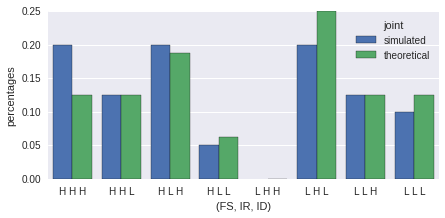
\includegraphics[width=1\textwidth]{figures/simplejoint.png}}
\caption{The limiting distribution of the simple treatment and an example frequency distribution pertaining to 400 random realizations.}
\label{fig:simplejoint} 
\end{figure}

But it is easy to see from a picture of the joint distribution describing joint behavior of the simple system (Figure \ref{fig:simplejoint}), for example, that very often three questions won't be needed. We could ask the person who knows whether the first variable, labeled ``Financial Sector'', has taken on the value ``H''.  If the answer is no, we could ask if the outcome is the event ``L'', ``H'', ``L'' and very often we would be right, finding the answer with only $2$ yes or no questions. Better yet, if we knew or somehow guessed the correct causal structure, we would know that whenever the ``Financial Sector'' variable takes on the value ``L'' and the ``Interest Rate'' variable assumes the value ``H'', the ``Industry'' variable must be in the low state. So, if we asked first ``is the value of the Financial Sector high'' and received ``no'' as an answer and then we asked ``is the value of the Interest Rate high'' and we received ``yes'' as an answer, we could be certain that the outcome must be ``LHL''. On average, for the simple system we would need to ask $2.7$ yes or no questions, if we know the distribution.   

\subsection{The Kullback-Leibler divergence}

The Kullback-Leiber Divergence was proposed as a measure of difference between two probability distributions $P$ and $Q$. Specifically, it was meant as a measure of the information that is lost when belief $Q$ is used as an approximation for a true probability distribution $P$:
\\

$D_{KL}(P(X) | | Q(X))=\sum_ip_i\log_2(\frac{p_i}{q_i}).$
\\

It is readily apparent that the Kullback-Leibler divergence can be re-expressed as follows:
\\

$D_{KL}(P(X) | | Q(X))=\sum_i (p_i\log_2p_i -p_i\log_2q_i = H(P, Q)-H(P)$, 
\\

where $H(P, Q)$ is known as the cross-entropy of $P$ and $Q$, and $H(P)$ is simply the entropy of $P$.

There are two problems with the Kullback-Leibler divergence as a measure of distance: 1) it is not symmetric ($D_{KL}(P | | Q) \not= D_{KL}(Q | | P)$) and 2) for the two distributions $P$ and $Q$, if one of the $q_i$ is equal to $0$, but the corresponding $p_i$ is not equal to $0$, the measure is not defined.  For example, we can see that when we simulated the complex process, some of the theoretically rare but possible outcomes have not yet occurred during the simulation and thus, if we want to measure the distance between the theoretical distribution and the frequencies of the simulated outcomes, using the Kullback-Leibler divergence, we will find that this measure is not defined. 

\subsection{The Jensen–Shannon divergence}

The Jensen–Shannon divergence is a symmetrized version of the Kullback-Leibler divergence that also solves the zero division problem:
\\

$D_{JS}(P | | Q)=\lambda*D_{KL}(P | | M) + (1-\lambda)*D_{KL}(Q | |M),$ 
\\

where $M=\lambda P + (1-\lambda) Q$ and $\lambda$ is usually, but not necessarily equal to $\frac{1}{2}$. In order for the measure to be symmetric, $\lambda$ has to be equal to $\frac{1}{2}$. 


The value of the Jensen-Shannon divergence is always between $0$ and $1$; $0$, when the two distributions are the same and $1$ when the two distributions have orthogonal support. This measure quantifies the amount of information in bits, about which of the two distributions one bit of data was drawn from, given that it was drawn from the first distribution with probability $\lambda$ and from the second with probability $1-\lambda$. For example, if the two distributions are the same, any bit of data will render no information about which of the two identical distributions it was drawn from, while if the two distributions have orthogonal support, each bit of data gives exactly one bit of information. To state this in Bayesian terms: if the two distributions are the same, then we can not learn from data and our posterior probability about which of the two distribution that data was drawn from is equal to our prior ($\lambda$ for the first distribution). At the other extreme, if the distributions have orthogonal support, the posterior will put probability $1$ on the distribution that supports the data; one bit of data carries one bit of information. 

\subsection{Cognitive Distance and the Performance Score}

If the square-root of the Jensen-Shannon divergence is taken, the result is a metric known as the Jensen-Shannon distance. This is the distance metric we use to calculate distances between any two distributions.  We refer to it as Cognitive Distance (CD):

\begin{equation}
CD(P, Q) = \sqrt{D_{JS}(P | | Q)}
\end{equation}

and to remind the reader, our performance score of person $i$ at time $t$, (supressing the index $i$), $S_t$, is 

\begin{equation}
S_t = 1 - CD(M_t, T),
\end{equation}

where $M_t$ is some person's Bayes Net model, at time $t$, of the true stochastic system, $T$. 


\end{document}




 


